\documentclass[12pt,a4paper]{bhamdissertation}

%load any additional packages
\usepackage[utf8]{inputenc}
\PassOptionsToPackage{hyphens}{url}
\usepackage[hidelinks]{hyperref}
\usepackage{amssymb}
\usepackage[UKenglish]{babel}
\usepackage[nodayofweek]{datetime}
\usepackage{pdflscape}
\usepackage{titlesec}
\usepackage[backend=biber,bibencoding=utf8,style=ieee,sorting=none]{biblatex}
\usepackage[toc,page]{appendix}
\usepackage{lipsum}
\usepackage{enumitem}
\usepackage{url}
\usepackage{minted}
\usemintedstyle{friendly}
\usepackage[autostyle]{csquotes}

\newcommand{\code}[1]{\texttt{#1}}

\titleformat{\paragraph}{\normalfont\normalsize\bfseries}{\theparagraph}{1em}{}
\titlespacing*{\paragraph}{0pt}{3.25ex plus 1ex minus .2ex}{1.5ex plus .2ex}

\title{Equaliser}
\author{George Brighton}
\college{School of Computer Science}
\degree{MEng Computer Science \& Software Engineering}

\addbibresource{references.bib}
\bibliography{references}

\begin{document}

%this baselineskip gives sufficient line spacing for an examiner to easily
%markup the thesis with comments
\baselineskip=18pt plus1pt

%set the number of sectioning levels that get number and appear in the contents
\setcounter{secnumdepth}{3}
\setcounter{tocdepth}{1}

\maketitle

\begin{romanpages}

\tableofcontents

% should be possible to move contents line to class file...
% http://tex.stackexchange.com/a/258973 for why 3 things are needed
\cleardoublepage\phantomsection\addcontentsline{toc}{chapter}{Abstract}
\begin{abstract}
Equaliser aims to prevent touts' exploitation of surplus demand for sought-after entertainment, which prevents genuine fans and supports from attending events at a fair price. The proposed solution encompasses the ordering process and mechanisms of venue entry, acting as a single end-to-end system for ticket distribution and validation. The software associates tickets with registered individuals at the point of purchase, forbidding all ticket transfer due to the inability to distinguish between friendly and malicious activity. It is observed, much to the author's disappointment, that verification of identity at venues that is both automatic and accurate is infeasible, resulting in manual validation that the photo assigned to the user matches the person in attendance. The solution is ultimately successful, with no known weaknesses, and is a viable replacement for other ticket distribution systems currently used by the industry.
\end{abstract}

\cleardoublepage\phantomsection\addcontentsline{toc}{chapter}{Acknowledgements}
\begin{acknowledgements}
This dissertation is the result of many useful and fruitful conversations. I am most indebted to Ian Batten for his boundless enthusiasm and limitless ideas, and for being very generous with his time, suggesting various angles of approach I would have never considered. Helen Crump deserves recognition for her patience in enduring my affair with the project over the past several months, and David Oswald kindly provided many useful areas to explore further during my inspection. Finally, I would like to thank the kind people at Twilio who provided a generous amount of credit to fund my two-factor authentication efforts.
\end{acknowledgements}

\end{romanpages}

\chapter{Introduction}

This report describes the design and implementation of a complete ticket distribution system that is immune to the £1B \cite{MF16} touting industry. Negative media coverage of the secondary ticketing market has reached a crescendo \cite{JR16}, and there are consultations in progress to ascertain whether, as happened to football in 1994, the reselling of entertainment tickets should be prohibited by law \cite{H15}. Regardless of the outcome, touts will continue to operate until a solution arrives that renders their business infeasible. This project aims to create that solution.

My intention was for the project to function similarly to a start-up in its first months of operating. There was no comprehensive solution to the issue of unauthorised ticket resale, so the majority of my efforts went into many hours of research, analysis, subsequent brainstorming and design. After completing this design, I then wanted to implement my own solution, and validate it accomplished what many companies with many thousands of employees were seemingly unable to achieve.

\section{Outline}

\begin{description}
    \item[\nameref{mining}] This chapter picks through an analysis of the current state of the art of ticket systems, their efforts to prevent touting, and their effectiveness at doing so. We shall also establish a set of metrics by which to judge a future ticket distribution system.
    \item[\nameref{requirements}] In this chapter, we formally organise metrics of successful systems into functional and non-functional requirements, resolving conflicts to produce a clear specification.
    \item[\nameref{practical_design}] This chapter provides insight into my decision making processes while developing the workings of the system at a high level. We go through these in chronological order, to provide insight into why the system works how it does in the final product.
    \item[\nameref{technical_design}] This chapter details my work in taking the practical design and investigating how best to turn it into a working system. We shall cover both the high-level architecture and individual interactions of key components to complete specific tasks.
    \item[\nameref{testing}] Here we discuss the principles employed to improve code quality and ensure correctness. I cover the challenges of testing an asynchronous codebase, and the system's continuous integration process.
    \item[\nameref{evaluation}] This chapter presents an analysis of the system, both in its own right, and compared to equivalent solutions on the market. We also discuss the project in relation to its original specification, and cover known deficiencies.
    \item[\nameref{applications}] The scope of the project was to solve the issue of touting, however the fundamental methodology is widely applicable. Here, we explore how it could be used in future across a variety of services, and the efforts required to adopt the system.
\end{description}


\chapter{Mining properties of existing systems} \label{mining}

The insights in this section are based on a whitepaper \cite{B17} I produced earlier in the project detailing the current state of the ticketing industry. As it is clear that there is currently no complete solution to the issue of touting, it qualitatively analyses the research in the paper to identify attributes that are conducive and resistant to touting, and other notable features whose absence or presence would enhance a future ticket distribution system.

\section{Single Distributor}

The practice of event organisers using multiple distributors is a blatant issue, as it allows any protections offered by a system to be circumvented by a vulnerable one. Malicious actors would simply use the latter. DICE identified this issue, and plugged the hole by making themselves the exclusive distributor of tickets for a given event \cite{D16}. If two systems existed in future that were secure in isolation, using them together could potentially also introduce issues or opportunities for confusion, so in practice, one distributor should always be used.

Box offices are inherently at odds with this observation on several levels. If a venue's box office is to be its sole distributor of tickets, using a separate system for each venue would be a great inconvenience to fans and event organisers. If we make the reasonable assumption that a box office alone cannot handle the demand for tickets, then another distributor is needed, which means the box office must be removed to maintain the single source. Unfortunately, from a touting prevention perspective, box offices are pointless at best, and a subversive side-channel attack at worst.

\subsection{Conflict of Interest}

Given the rule of a sole distributor, companies will compete to win the business of being that distributor. To differentiate themselves, these firms can highlight the rate at which they sell tickets, and the total number of tickets sold, which may conflict with ensuring those tickets go to genuine fans. This can only be solved by removing all metrics related to the rate of ticket sales from a distributor's fee calculation. They should receive a fixed payment that is agreed in advance and independent of the number of tickets sold. Promotion must be distinct from processing.

\section{Ticket Transferability}

Paper tickets are inherently broken, as it is impossible to prevent the transfer of a physical object between parties. Adding a name which is rarely validated does nothing to improve the situation. Paperless tickets were ostensibly introduced to combat ticket transfer, with the addition of photo ID \cite{B07} verification a key improvement, however as already discussed, only the purchaser's identity is validated (if at all), leaving 3-7 tickets per credit card available for touting, and a tidy profit. Unfortunately, DICE is ineffective against touts in this regard. If an individual buys several tickets, there is nothing tying these to individuals, hence they can be resold.

Automation of the ticket purchasing process attacks the same vulnerability, and the reCAPTCHA \cite{T167} test used by Ticketmaster and others is duct tape over a deeper problem. A system that is vulnerable to bots is also vulnerable to humans, if to a lesser extent. Limiting the number of tickets that can be purchased per transaction is another smoking gun, and has only resulted in touts using multiple credit cards \cite{DJ16}. The only way to truly fix these two issues is to address the transferability problem.

The entire reselling industry only exists because tickets are, in practice, transferable. Twickets \cite{Tw161} is well-intentioned, but by focusing exclusively on the secondary market makes itself part of the problem. It should not be possible for tickets to go near a secondary ticketing site, as touts are under no obligation to use a benevolent one. Therefore, the solution is for an identity to be tied to a ticket, and validated on entry to the venue.

\subsection{Reallocation}

Ticket reallocation occurs when an individual with a ticket wants to return it for a refund. DICE made the key design decision to not allow the purchaser any say in who returned tickets go to. By simply returning tickets to a pool, a tout cannot resell a ticket, as they have no control over who receives it. In a system that identified every ticket holder, this would be a useful property, however unfortunately, due to the aforementioned issue with only validating the purchaser's identity, it is redundant for DICE. As tickets are nameless, a tout can replace those he lets in as many times as he likes before the event. 

\section{Notable Features}

In addition to properties directly related to the prevention of touting, it is useful to note ways in which these systems are either suboptimal or successful.

\subsection{Purchase Timeout}

The concept of entering a minimal set of details, then having a fixed amount of time to complete the purchase is very useful. It levels the playing field, meaning people are not penalised for being slow at typing or mis-entering payment information. It also reduces the amount of time users are under pressure for, without hindering competition, leading to a more pleasant ordering experience.

\subsection{Stability}

Ticket websites fall over with such predictability during large releases \cite{B10} that one would be forgiven for thinking it were a requirement. Since the introduction of cloud computing several years ago, there has been no excuse for being unable to handle spikes in demand. Any ticket vendor that meets the seemingly straightforward criterion of staying online during a large release would already be ahead of the competition.

\subsection{Group Entrance}

Due to the way paperless tickets work, all members of a group must enter the venue at once \cite{T166}. While not broken entirely, this can cause serious inconvenience if one person in a large group is running late. A secondary issue here is that of gifted tickets. As the payment card is effectively the ticket, it is not possible to buy tickets for two friends to attend an event on their own \cite{T166}. Each person in a group should be able to enter the venue in their own right. This should not be a challenging requirement if each ticket is individually tied to a person.

\subsection{Fees}

Fees are one of the most disliked properties of existing systems \cite{P12}, yet one of the easiest to fix. It is clear that current fees are not related to their label, the most obvious example being Ticketmaster charging for delivery of tickets sent via email \cite{P12}. Customers know they are used to maximise revenue while keeping the perceived price of tickets as low as possible.

Removing these fees is obviously the ideal, but a more pragmatic solution would be to include them in the ticket price, so buyers see a single value. This would be more popular with customers, as it is more honest. The increase in face value will not put people off or leave a sour taste nearly as much as a list of questionable charges. DICE succeeded in this regard by showing no fees to purchasers, and buyer perception is amongst the highest of any distributor \cite{D16}.

\chapter{Requirements} \label{requirements}

Analysis of the current state of the art with regard to ticket touting provided a ruler by which to measure any new ticket system. By flipping this on its head, I hoped to use these metrics to design core requirements for a perfect system. Many more requirements would emerge during the practical design, however they were not perceived in advance, simply because no system so far was able to offer a complete solution to ticket touting.

\section{Functional}

\begin{enumerate}
    \item Users should be able to return a ticket for a refund.
    \begin{enumerate}
        \item This should be permitted outright, or only if the system can reallocate those tickets to someone in the waiting list, so no revenue is lost.
    \end{enumerate}
    \item Direct ticket transfers between individuals should not be permitted. User A should not be able to give their ticket to User B, as we cannot prevent money from changing hands outside of the application.
    \begin{enumerate}
        \item Unwanted or refunded tickets should be returned to a pool of available tickets.
    \end{enumerate}
    \item Users should only have to enter a minimum number of details before their tickets are reserved, or they enter the waiting list.
    \item Venue staff must be able to re-validate a ticket and verify an attendee's identity inside the venue.
    \item Two-factor authentication should be mandatory for login.
\end{enumerate}

\subsection{Groups}

\begin{enumerate}[resume]
    \item Each ticket in a group booking must be tied to a registered user at the point of order.
    \item Each attendee in a group should be able to enter the venue individually on their own merit.
    \item A group leader must be able to specify that some members in a group should pay for their own tickets.
\end{enumerate}

\subsection{Gifts}

\begin{enumerate}[resume]
    \item A user should be able to purchase tickets for others.
    \item They should be able to individually specify when those tickets should become visible to the giftees.
    \item The gifter should be able to attach a message to each gifted ticket that will be displayed when it is revealed to the giftee.
    \item The gifter can refund a ticket before it is released to the giftee, after which only the giftee can refund it.
    \item The original purchaser is always refunded the cost of the ticket, even if a giftee initiates a refund.
\end{enumerate}

\section{Non-functional}

\begin{enumerate}[resume]
    \item The system must partner with event organisers to be the one and only distributor of tickets. Only tickets issued by the system and verified by staff upon entry should be accepted.
    \item Fees should be included in the cost of the ticket.
    \item The ordering system should be able to support 500,000 simultaneous users.
    \item No subsystem should have a single point of failure.
\end{enumerate}

\chapter{Practical Design} \label{practical_design}

My task was now to design a ticket distribution system using the requirements in the previous chapter as non-negotiables. Even with these constraints, it was difficult to know where to start. Ticket distribution is not particularly expansive or complex, but I was well aware that touts' livelihoods depend on circumventing any protections I put in place, so if there were any weaknesses, they would be found. If my design turned out to be flawed, it would be no better than any other existing solution.

\section{Entrance}

I decided to start by focusing on the process by which ticket holders would gain access to a venue, as controlling this is ultimately the main purpose of the system. If at all possible, I wanted this to be completely automatic, with no human verification needed. This would remove any chance of human error or corruption, while making my solution more attractive to venues, who would not have to hire as many staff.

To make this work, I knew I would have to produce a token that could only be used by its rightful owner to enter a venue. At first, I considered payment cards, for the reason that many experts have already put a lot of effort into making these secure. Unfortunately, this had two key problems.

\begin{enumerate}
    \item In a group scenario, only the original purchaser necessarily has a payment card on file. As the system would not know about the cards of anyone else in the booking, they would have to enter the venue together, which was a direct violation of the requirements.
    \item Requiring each individual to have a payment card on file is too draconian. Not everyone going to an Ed Sheeran concert is old enough to own a credit card, and it is unreasonable to require parents to give them to their children - and even then, there is only one copy of the card.
\end{enumerate}

This was clearly unworkable. By going through this process, I knew the token had to be something that everyone would have, and for convenience, preferably something they already carried with them. The most obvious choice was a mobile phone, which has the added benefit that I could put arbitrary data on it to act as a ticket. It is trivial to send and receive data via the internet, and as phones have a screen, they could display this data however I liked, which could be the same as existing ticket barcodes so no changes to ticket barriers would be required.

I quickly thought of a handful of ways that a barcode could be displayed on a phone securely. It could be a hash of some key material unique to the user, such as an X.509 private key. An intermediate certificate authority could be created for each event, that would sign requests for tickets. If a refund was initiated, the ticket could be revoked and so on. To make tickets difficult to copy, the key material could be hashed with a timestamp every 30 seconds, and an animation could be displayed to make it difficult to screenshot. This was not perfect, but the pace at which I was able to generate possibilities made me reasonably confident of being able to tie a ticket to a phone.

Unfortunately, it was all for nothing. It is one thing to tie a ticket to a phone, but it is quite another to ensure the person who shows up to a venue with that phone is its true owner. Any number of security features are all irrelevant if a tout can simply give a phone containing a ticket to someone else. Indeed, touting is so lucrative that one could quite easily buy 10 or 100 pay-as-you-go phones and include the cost of the phone in the price of the ticket. This problem turned out to be much harder than initially thought.

At first, I considered forcing the user to enter a passcode, however I realised the challenge cannot be based around knowledge, as that can be transferred from the tout to their buyer. Similar to the ideas behind two-factor authentication, it requires something you have, not something you know. I then looked into biometrics, for example using a fingerprint to reveal the barcode for a few seconds at the barrier, under the assumption it would be too awkward and obvious for a tout to pass this challenge before letting in someone else. Unfortunately, there were four issues.

\begin{enumerate}
    \item Although becoming more prevalent, many phones are not equipped with fingerprint readers, and of those that are, only 15\% of owners bother to set it up \cite{B16}. Relying on such technology would require a two-lane system where those with less-able phones would queue. Any malicious actors would simply use the weaker security.
    \item Even amongst phones with the technology, they do not always function correctly. A 1\% mis-read rate equates to 900 people at Wembley Stadium, which is unacceptable.
    \item The phone is literally in the hands of the attacker, and biometrics fundamentally trust the phone's technology. Ideally, I only wanted to have to trust what is under my control.
    \item On iOS, applications receive a boolean response to a fingerprint scan. They cannot identify who a fingerprint belongs to \cite{G16}, so an attacker could simply register the fingerprint of whoever bought a touted ticket, and the ticket app would be none the wiser.
\end{enumerate}

I decided the technology was neither secure nor reliable enough to use. I also considered photographs, which could be recognised at the barrier, but again the technology lacks accuracy.

Disheartened that phones alone were not the opportunity I thought they were, I moved to using them in combination with another form of identity. I briefly revisited credit cards as a possible option, particularly because they are not something given to a stranger lightly, but at the same time touts are known to own many cards, and could make buyers pay a deposit. I kept reminding myself that it was in both the tout and their customers' interests to outsmart the system; the threat model cannot assume any customer is trustworthy.

Passports seemed to be more promising, however they are almost too valuable. I struggled to come up with a document that was private enough to be worth validating, but not so private as to worry genuine purchasers. Thefts are common at concerts \cite{C10}, and crime would only increase if thieves knew everyone in attendance had a credit card, smartphone and passport on them.

Photocards and Oyster cards initially seemed to be an answer. They are difficult enough to get hold of and a pain to replace, however they are bespoke to each country (in the case of Oyster, a single city \cite{O17}), and sometimes even genuine copies look fake. The real issue was that they are trivially easy to photocopy, and many countries, such as Germany, do not allow non-governmental organisations to use national identity cards \cite{M11}. Any automated system is vulnerable to forgeries. Without a human present to check each document, I had no reliable defence against this.

\subsection{Manual Verification}

Regretfully, I resigned to having humans at the turnstiles to verify attendees. I took comfort in the fact that passport gates at the UK border still require a human to confirm access \cite{Ba16}. If even these are not entirely automatic, when in complete control of the physical token (the passport), the chances that I would be able to come up with a secure solution were little to none. This was a disappointment, but no worse than the current paperless system.

To reduce the likelihood of staff intimidation, it could be done in a similar fashion to passport gates, where staff are kept physically separate from the people they are allowing through. To limit potential issues of corruption, where a member of staff lets their friends through, two controllers could manage several lanes, with individual requests for entry being randomised between them, so there was no guarantee of being confirmed by a single person. Regardless, this has the benefit of not requiring one employee per lane into the venue, so the increase in cost is not as substantial as I thought.

My attention then turned back to the exact checks to perform. Photos were showing the most promise, and humans are good at comparing faces, so I revisited this idea. I envisaged a system where users would upload a photograph of themselves during registration, which would be shown alongside the barcode. A human would then ensure the person in front of them matched, and allow them through.

Photos would have to be vetted to make sure they were appropriate, however this could be done automatically to some extent. Facial recognition could be used to verify that one and only one face appeared in the image, and it was of appropriate size. Ultimately, such a mechanism may need a human to confirm, however this would only have to be done once per person. Of course, the photo would have to be verified before any tickets were allocated, and could not be changed at will. Any updates would have to be approved to ensure the person in the photo was the same. Ticketmaster has a similar verification system for the case where the payment card expires before an event \cite{T166}.

I was happy with all of this, apart from the photo existing on the user's phone, which felt dangerous - as already mentioned, the phone is in the hands of Mallory. To remove this dependency, I decided that, instead of showing the photo on the phone when the barcode was scanned, the system would show the photograph on file alongside the attendee, then the member of staff would simply accept or reject entry. This had the nice property that all ticket material on the phone need no longer be secure, as even armed with another person's ticket, it would not be possible to pass the visual check (identical twins notwithstanding, but they are unlikely to tout to each other). Not relying on the phone is a strong definition of security. There was no longer any value in mimicking someone else's phone, so I would not have to put lots of effort into countermeasures.

The outcome was realising the phone is effectively reduced to a pointer to a person, like a user ID. To mitigate the risk of attackers iterating through all users, attempting to find people who looked similar to each other, I decided to make the token long and random, so it is infeasible to explore the entire space. As the number of possible user IDs grows, the likelihood of any single one pointing to an actual person approaches 0.

Therefore, in summary, when a user registers, they upload a clear photo of themselves. They have a single ``ticket'' for all events, which is unique to them. Upon scanning this data at the ticket barrier, their profile is retrieved, and automatically checked to see whether they have a valid ticket for the event. If they do, a member of staff compares the photo on file with the person who has shown up. If they match, the person is allowed in. A given person is only allowed in once. As tickets in themselves are useless for entry, they cannot be touted. Even changing the barcode is unlikely to point to another user, and even if it does collide, the chances are astronomically small that the face will resemble the attacker's, or even have a ticket. Tokens can also be regenerated regularly completely automatically, without users noticing.

\section{The Event Hierarchy}

At this stage, I started confusing myself. An ``event'' could refer to ``Wimbledon'', ``Wimbledon 2017'', ``Wimbledon 2017, Day 1'', or ``Wimbledon 2017, Day 1, Centre Court''. Some more accurate vocabulary was needed to avoid ambiguity.

\begin{description}
    \item[Tiers] A type of ticket for a single performance, e.g. \textit{Standing}, \textit{Stalls}, or \textit{Debentures}. A tier has an associated price, availability and returns policy (always, or only if the ticket can be reallocated). It may or may not have a seat allocation.
    \item[Fixtures] Generally, a fixture will match the duration of a ticket's validity, e.g. \textit{UKNOF 38} or \textit{Wimbledon 2017, Day 4, Centre Court}. Fixtures have a designated venue, and one or more tiers.
    \item[Series] Fixtures combine to form series, which are collections of experiences, usually over no more than a couple of months. Examples include \textit{Glastonbury 2017}, \textit{Derren Brown: Svengali}, and \textit{Ed Sheeran: X Tour}. Their start and end dates can be derived from the fixtures within them.
    \item[Headlines] I considered this final tier to contain series, however they were ultimately not implemented, in favour of tags instead. Examples would have been \textit{Wimbledon} and \textit{6 Nations}.
\end{description}

I wanted the system to be able to handle as many types of event as possible, so generic terminology was needed. However, it need not be exhaustive. If a new type of event that does not fit the above structure came along, I decided the event organiser could adapt and, if necessary, abuse the hierarchy to fit their needs. Ticketmaster is a frequent culprit in this regard.

\section{Etymology}

I was now beginning to see the system's role more clearly, and decided to call it \textit{Equaliser}. This had the nice property of applying to many different events, similar to the system, e.g. a mixing equaliser in the context of music, or an equaliser in a tennis match. I also saw it as a way of getting \textit{equal} with touts.

\section{Ordering}

I now had some requirements for the registration process, and a robust way to ensure only those with valid tickets could enter a venue. Now I needed to work out how to join these two together, i.e. how registered users could obtain tickets.

\subsection{Individuals}

I decided to tackle the case of an individual attending a fixture alone first, as it does not involve the co-ordination required for groups. The initial stages of this practically designed themselves:

\begin{enumerate}
    \item The user chooses the series, fixture and tier they are interested in.
    \item The user submits this order.
    \item If a ticket is not available for that tier, the user enters the queue and waits until it is available.
    \item If and when the ticket becomes available, the user is alerted and has a set amount of time to pay; if payment is received within this time, the ticket is delivered to their phone, otherwise their order is cancelled.
\end{enumerate}

I deliberated how long to allow for payment for quite some time; it was a compromise between keeping the waiting list ticking over, and preventing frustration caused by users missing out by minutes. Eventually, I decided to allow up to 30 minutes, with the potential for a shorter window as the event gets closer or the waiting list longer. In order that users would not be disturbed at uncommon hours, this limit only applies between 9am and 9pm; if a ticket becomes available outside these times, the user should have until 9:30am to pay. If a ticket does expire, the user could be sent to the back of the queue, but there is no guarantee that they will not miss it again, so rather than have them cycle through the queue, it is clearer to cancel their order. Anyone who truly wanted to attend would not miss their chance to pay for their ticket in the first instance.

\subsection{Fees}

Transactions made through the online shop will be paid into Equaliser's bank account. Event organisers will receive their majority share of that as agreed, with the venue also receiving a cut. It is no hardship to negotiate these fees, as the venue, event organiser and Equaliser already have to partner to prevent other ticket distributors allowing the system to be bypassed.

\subsection{Waiting List}

The fact that a ticket may not be available immediately complicates matters, but Equaliser would be fairly useless if it could not handle this situation. Tickets may become available either through refunds, or if ticket release is staggered. Intuitively, as tiers can sell out individually, I envisaged one waiting list per tier, however after deliberation, I found some subtle problems:

\begin{enumerate}
    \item A user may not care which tier they receive; they may just want to attend the event at all costs, i.e. any tier. With one waiting list per tier, the only way to implement this is to allow a user to be in multiple queues. It is fundamentally wrong to have a single user with two tickets, so this would introduce concurrency challenges to ensure a user only received one ticket, should they happen to be at the front of two waiting lists simultaneously.
    \item If an order is placed at the tier level, a user would have to place one order per tier, which is outrageous from a user-experience perspective, and makes it much harder to keep track of attendees and ensure no one receives two tickets.
\end{enumerate}

For these reasons, I decided instead to have one waiting list per fixture. Anyone who wanted sold out tickets would join this waiting list, and be able to indicate not only what tiers they were interested in, but also their order of preference. For example, an individual may choose to accept either dress circle or stalls tickets, with a preference for the stalls if both become available at the same time.

The allocation algorithm begins by finding which tiers are available, and how many tickets remain in each. It then walks down the queue, querying each person's order. If it can satisfy the demand, it makes the individual an offer, before decrementing the number of tickets for the fulfilled tier. Most importantly, in order to remain fair, the algorithm must not be able to discover new tickets mid-execution (as people already passed over may have wanted those tickets); it instead has to run periodically.

I considered giving users an indication of their position in the waiting list, either an absolute number, or estimated time to the front, however this could encourage abuse. Although contrived, a tout knowingly at the front of the queue could demand money for dropping out if they knew someone was behind them. In fact, it is difficult to provide any sort of metric that is no exploitable. The queue must behave like a dark pool in trading.

\subsection{Refunds}

Payment is not taken until an offer of a ticket is accepted. There are two refund policies offered by the system:

\begin{description}
    \item[Always] Refunds are always accepted and processed immediately.
    \item[Reallocate] Refunds are only processed when the system can give the ticket to someone else, in order to protect the event organiser's revenue. New tickets will always be used to fulfil demand before returned ones, therefore refunds that fall into this policy will only be accepted if there is a waiting list for the tier.
\end{description}

I considered a third option, \textit{never}, however there is no advantage to this over \textit{reallocate} for any stakeholder. It would not affect the event organiser, as they receive the revenue either way, yet it would be worse for the performer, as someone would be forced to attend who did not want to go. In practice, this could lead to empty seats, which is bad publicity.

\subsection{Groups}

Now that single tickets were worked out, I attacked the issue of scaling this to groups, which meant revisiting all of the challenges I went through to handle individuals. This was a deliberate decision, as the leap from nothing to groups would have been somewhat overwhelming. I was glad to have a solid foundation in the form of single orders to adapt. I found it much easier to keep something working and expand on it rather than handle so many more variables. The challenges included:

\begin{itemize}
    \item The fact that groups need to be treated as an individual unit of allocation. They cannot complete checkout in isolation, as there would be no guarantee of everyone succeeding in receiving a ticket.
    \item The concept of gifts, where it is not always simple to indicate or represent who pays for who, which is compounded in the case of refunds.
    \item The requirement that at no point can one person own multiple tickets, however this is at odds with the concept of a single order.
\end{itemize}

Firstly, I had to decide whether to impose a limit on the size of groups. Existing systems impose an upper bound to prevent abuse, however given ticket transfers are prohibited, there is no advantage to Equaliser having such a constraint. It was noticeable how properly solving the core problem of transferability allowed me to strip out many of the workarounds and duct tape that had been applied to other systems. Spending time on a few key decisions was paying dividends and saving a vast amount of complexity.

\subsubsection{Ordering Process}

% order individually
Next, I had to ensure all members of a group received tickets at the same time, or not at all. My first attempt involved people explicitly defining dependencies when making an order, for example person A specifies that they only want a ticket if persons B and C also get one; person B specifies they only want one if A and C receive one and so on. There were two key issues with this system:

\begin{enumerate}
    \item If everyone is forced to buy a ticket individually, they would have to co-ordinate seat selection and so on, all while others are doing the same. The chances of frustration are high, especially for popular events.
    \item It could be very complicated to calculate the dependencies when doing the allocation, particularly if the graph of members is not fully connected.
\end{enumerate}

% one on behalf of group
More simply, this method was just too complicated to ask users to understand, and would cause too many errors. I needed something more high-level and intuitive, and quickly realised the only sane way of doing this involved one person placing an order on behalf of the entire group. In the case of fixed seating, this would make it much easier to allocate a contiguous block of seating, and also creates a simple blob for the allocation system to fulfil or ignore. Having one person in charge also reduces confusion in case of issues, and also load on the system. There is no advantage to everyone in a group simultaneously trying to buy tickets to increase the likelihood of ``getting through''.

% now an issue of ownership; can associate with people at time of order
The issue with this was that of a single person owning many tickets. I needed a way to distinguish between someone genuinely purchasing tickets for friends, and someone who buys with the intention of touting. It took me far too long to realise that the key difference, and what is exploitable here, is that the person buying tickets for friends knows who those people are at the point of purchase. Whoever placed the order could enter friends' details, set who they wanted to pay for, and never be in control of any distribution.

% enter after offer received? no, before
To maintain the property of minimising the amount of information required before a user can join the waiting list, at first I decided to allow the group leader to enter names of attendees after an offer has been received. However, if a user had already purchased a ticket, this would mean it was not detected until after purchase, and secondly it would give touts a window to advertise that they had received tickets and solicit buyers. I realised it is more subtle and stricter than a genuine buyer knowing attendees at the point of purchase; to prevent the above, a buyer would have to specify who would attend before even knowing whether they had tickets. Therefore, in order to place an order, the group leader specifies a tier and a list of attendees, all of whom must already be registered with a validated photo. This is so the ticket cannot be touted and the buyer's photo added later. As part of the order processing workflow, a check would be made to ensure no users already had an active order for the fixture, to avoid the issue of multiple tickets per user.

\subsubsection{Waiting List}

Groups can share the current waiting list for individuals. Instead of allocating a single ticket, the algorithm simply passes over the group until a sufficient number are available. There are two potential issues here.

\begin{enumerate}
    \item If the amount of time between allocations is too short, not enough tickets will have accumulated to fulfil larger orders. A group of 8 at the front of the queue may never be served if the average rate of return is 8 tickets per minute, and the algorithm runs once every 30 seconds.
    \item It can be assumed that in the case of reserved seating, groups will want to sit together.
\end{enumerate}

To solve the first issue, the allocation algorithm could potentially analyse the rate of ticket returns, and determine whether it can wait long enough to fulfil a large order, e.g. if 1 ticket is returned every minute, it could wait 5 minutes to fulfil an order of 5. There would have to be a threshold on this to ensure turnover in the queue. Certainly, it should never be the case that smaller groups are not able to attend because the allocator is causing a log jam to satisfy a large group.

The second issue is made more complicated by the fact that existing orders cannot be moved around. All that can be done here is for the allocator to group tickets where possible (e.g. seats C23 and C24 would be a pair). It would then sort the size of these groups in ascending order, and starting at the front of the queue, try to find the smallest block size that would satisfy the order. This algorithm could be adapted depending on the type of seating available. The clear downside is that it would require detailed and accurate plans of all venues with reserved seating, however on the contrary, current ticket retailers must have these anyway.

\subsubsection{Payment}

The final issue is that of payment, which also implicates gifted tickets. As one person places the order, my initial idea was to have them pay for everyone for simplicity, then when a friend confirms the purchase, charge their payment card for the amount for their ticket, and do a partial refund for the buyer. Taking a step back, I realised this was again far too convoluted, and it is unreasonable to expect the buyer to be out of pocket, or even have enough money in their account for everyone if they only want a single ticket. There is also the issue of what happens if someone rejects their ticket. I definitely wanted to remove refunding from the normal payment workflow, as it incurs additional card processing fees.

To address all of these problems, I created a solution based on the idea of delegating responsibility for payment. A user wants to order $t$ tickets, of which $o$ are for other people, with $g$ of those gifted. $t - o$ will be $0$ if the group leader is not attending, or $1$ if they are. They will pay for $(t - o) + g$ tickets, with $o - g$ others paying for their tickets individually. Example scenarios include:

\begin{itemize}
    \item A user orders a ticket for himself.
    \begin{itemize}
        \item $t = 1, o = 0, g = 0$
        \item User pays for $(1 - 0) + 0 = 1$ ticket
    \end{itemize}
    \item A user orders a ticket for herself and 4 friends.
    \begin{itemize}
        \item $t = 5, o = 4, g = 0$
        \item User pays for $(5 - 4) + 0 = 1$ ticket
    \end{itemize}
    \item A user orders a ticket for himself and 4 friends, 2 as gifts.
    \begin{itemize}
        \item $t = 5, o = 4, g = 2$
        \item User pays for $(5 - 4) + 2 = 3$ tickets
    \end{itemize}
    \item A user orders 2 tickets for her children, both as gifts.
    \textit{N.B. she is not attending the event.}
    \begin{itemize}
        \item $t = 2, o = 2, g = 2$
        \item User pays for $(2 - 2) + 2 = 2$ tickets
    \end{itemize}
\end{itemize}

I intuitively saw several roles emerging here. An order consisted of a set of transactions, with each of those transactions paying for one or more tickets. The total number of transactions for an order will be $t - g + (1 - (t - o)) = o - g + 1$. A transaction's payee may not even be paying for his own ticket. Some new terminology was in order:

\begin{description}
    \item[Group leader] The user who places an order. They may not necessarily be paying for anyone.
    \item[Payment group leader] A user paying for one or more others, possibly themselves.
    \item[Attendee] Someone attending a fixture.
\end{description}

\chapter{Technical Design} \label{technical_design}

I now had a clear idea of how the system would function, so it was comparatively easy to implement this in code. I adopted a top-down approach, starting with the self-contained systems that combine to form Equaliser.

\section{Architecture}

At the highest level, there would be two types of user: venue staff and customers. Both could potentially need to use a variety of devices, so I wanted to design Equaliser such that the exact front-end was irrelevant. The obvious solution to this is the client and server model, used by many modern applications including Twilio, Travis CI and GitHub, where an API is exposed by a core service, and then consumed by other clients. It quickly became apparent that, while the clients used by staff at the barriers were a crucial component, they were relatively trivial to implement compared to the customer-facing parts, partly by virtue of being read-only. In the interest of spending time on the more challenging issues, I decided to account for, but not implement this part of the system.

I knew a a mobile phone was necessary to use the system, which left the choice of either a native client, or website. In order to demonstrate any API's ignorance of client, there had to be at least two, so I decided to implement both. As I was familiar with Java, but had no experience or facilities to develop for the iPhone, I targeted Android for the native client. Therefore I would implement three components:

\begin{description}
    \item[API] The backend of the entire application, maintaining all state, and exposing a JSON REST interface for other parts to interact with.
    \item[Mobile app] A native API front-end for Android, which uses the API directly.
    \item[Website] Another front-end for generic web browsers.
\end{description}

\begin{figure}[ht]
    \centering
    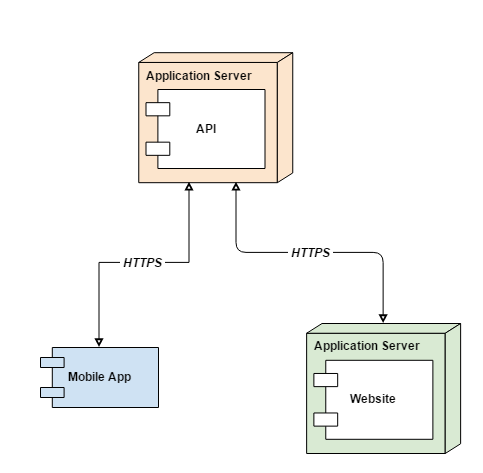
\includegraphics[resolution=120]{img/architecture.png}
    \caption{Equaliser deployment diagram}
\end{figure}

\section{API}

A self-imposed requirement of the project was to be able to handle 500,000 concurrent users hitting the order page. In order to achieve this, I knew the API would have to both make efficient use of hardware while being able to scale out. I initially considered Node.JS, however this does not scale well to multiple cores well due to its single event loop. I had heard of Vert.x \footnote{\url{http://vertx.io/}}, another reactive framework during my placement year, and this seemed like a perfect match and learning opportunity. I knew that Equaliser would not be a typical web application that simply reacted to incoming requests. Various background processes were needed for tasks like waiting list allocation, and Vert.x includes ``verticles'', which run independently and communicate using an event bus, which I found makes communication within a cluster trivial. Even while reading through the documentation, I found myself planning how to map Equaliser into Vert.x.

\subsection{Performance}

Vert.x is special in that, bar a handful of filesystem-related methods, it is entirely asynchronous. This allows it to deal with a high amount of concurrency using very few kernel threads, by avoiding blocking calls. Where a normal framework's methods would block if necessary and return a result, almost all methods in Vert.x return \code{void} and instead take a callback. A system can only have a few thousand threads before it grinds to a halt, which sets an upper limit on the number of users that can be handled using a normal synchronous model. Vert.x was a great way to ensure Equaliser was capable of saturating whatever hardware it does run on.

\subsection{Database}

The API itself would obviously require some form of database. I considered using a NoSQL database such as MongoDB, however, particularly as Equaliser is effectively a shop, the lack of transactions was unworkable. Therefore, I decided to use MySQL, for the simple reasons that its driver is Vert.x's most mature, and the system itself is well known by many developers.

Before writing any application code, I designed the schema for the database. An EER diagram of the final version can be found in Figure \ref{fig:database}. This was effectively a write up of the practical design. Surprisingly, on several occasions I found that the table structure could be simplified by being made more flexible. For example, according to the system design, only a group leader must be able to gift tickets. However, it turns out that this special case makes the schema more complex, so I decided to support any number of payment groups containing any number of attendees. This had the rare advantage of both removing complexity and adding functionality.

\begin{landscape}
    \thispagestyle{empty}
    \begin{figure}[p]
        \vspace*{-2cm}
        \makebox[\linewidth]{
            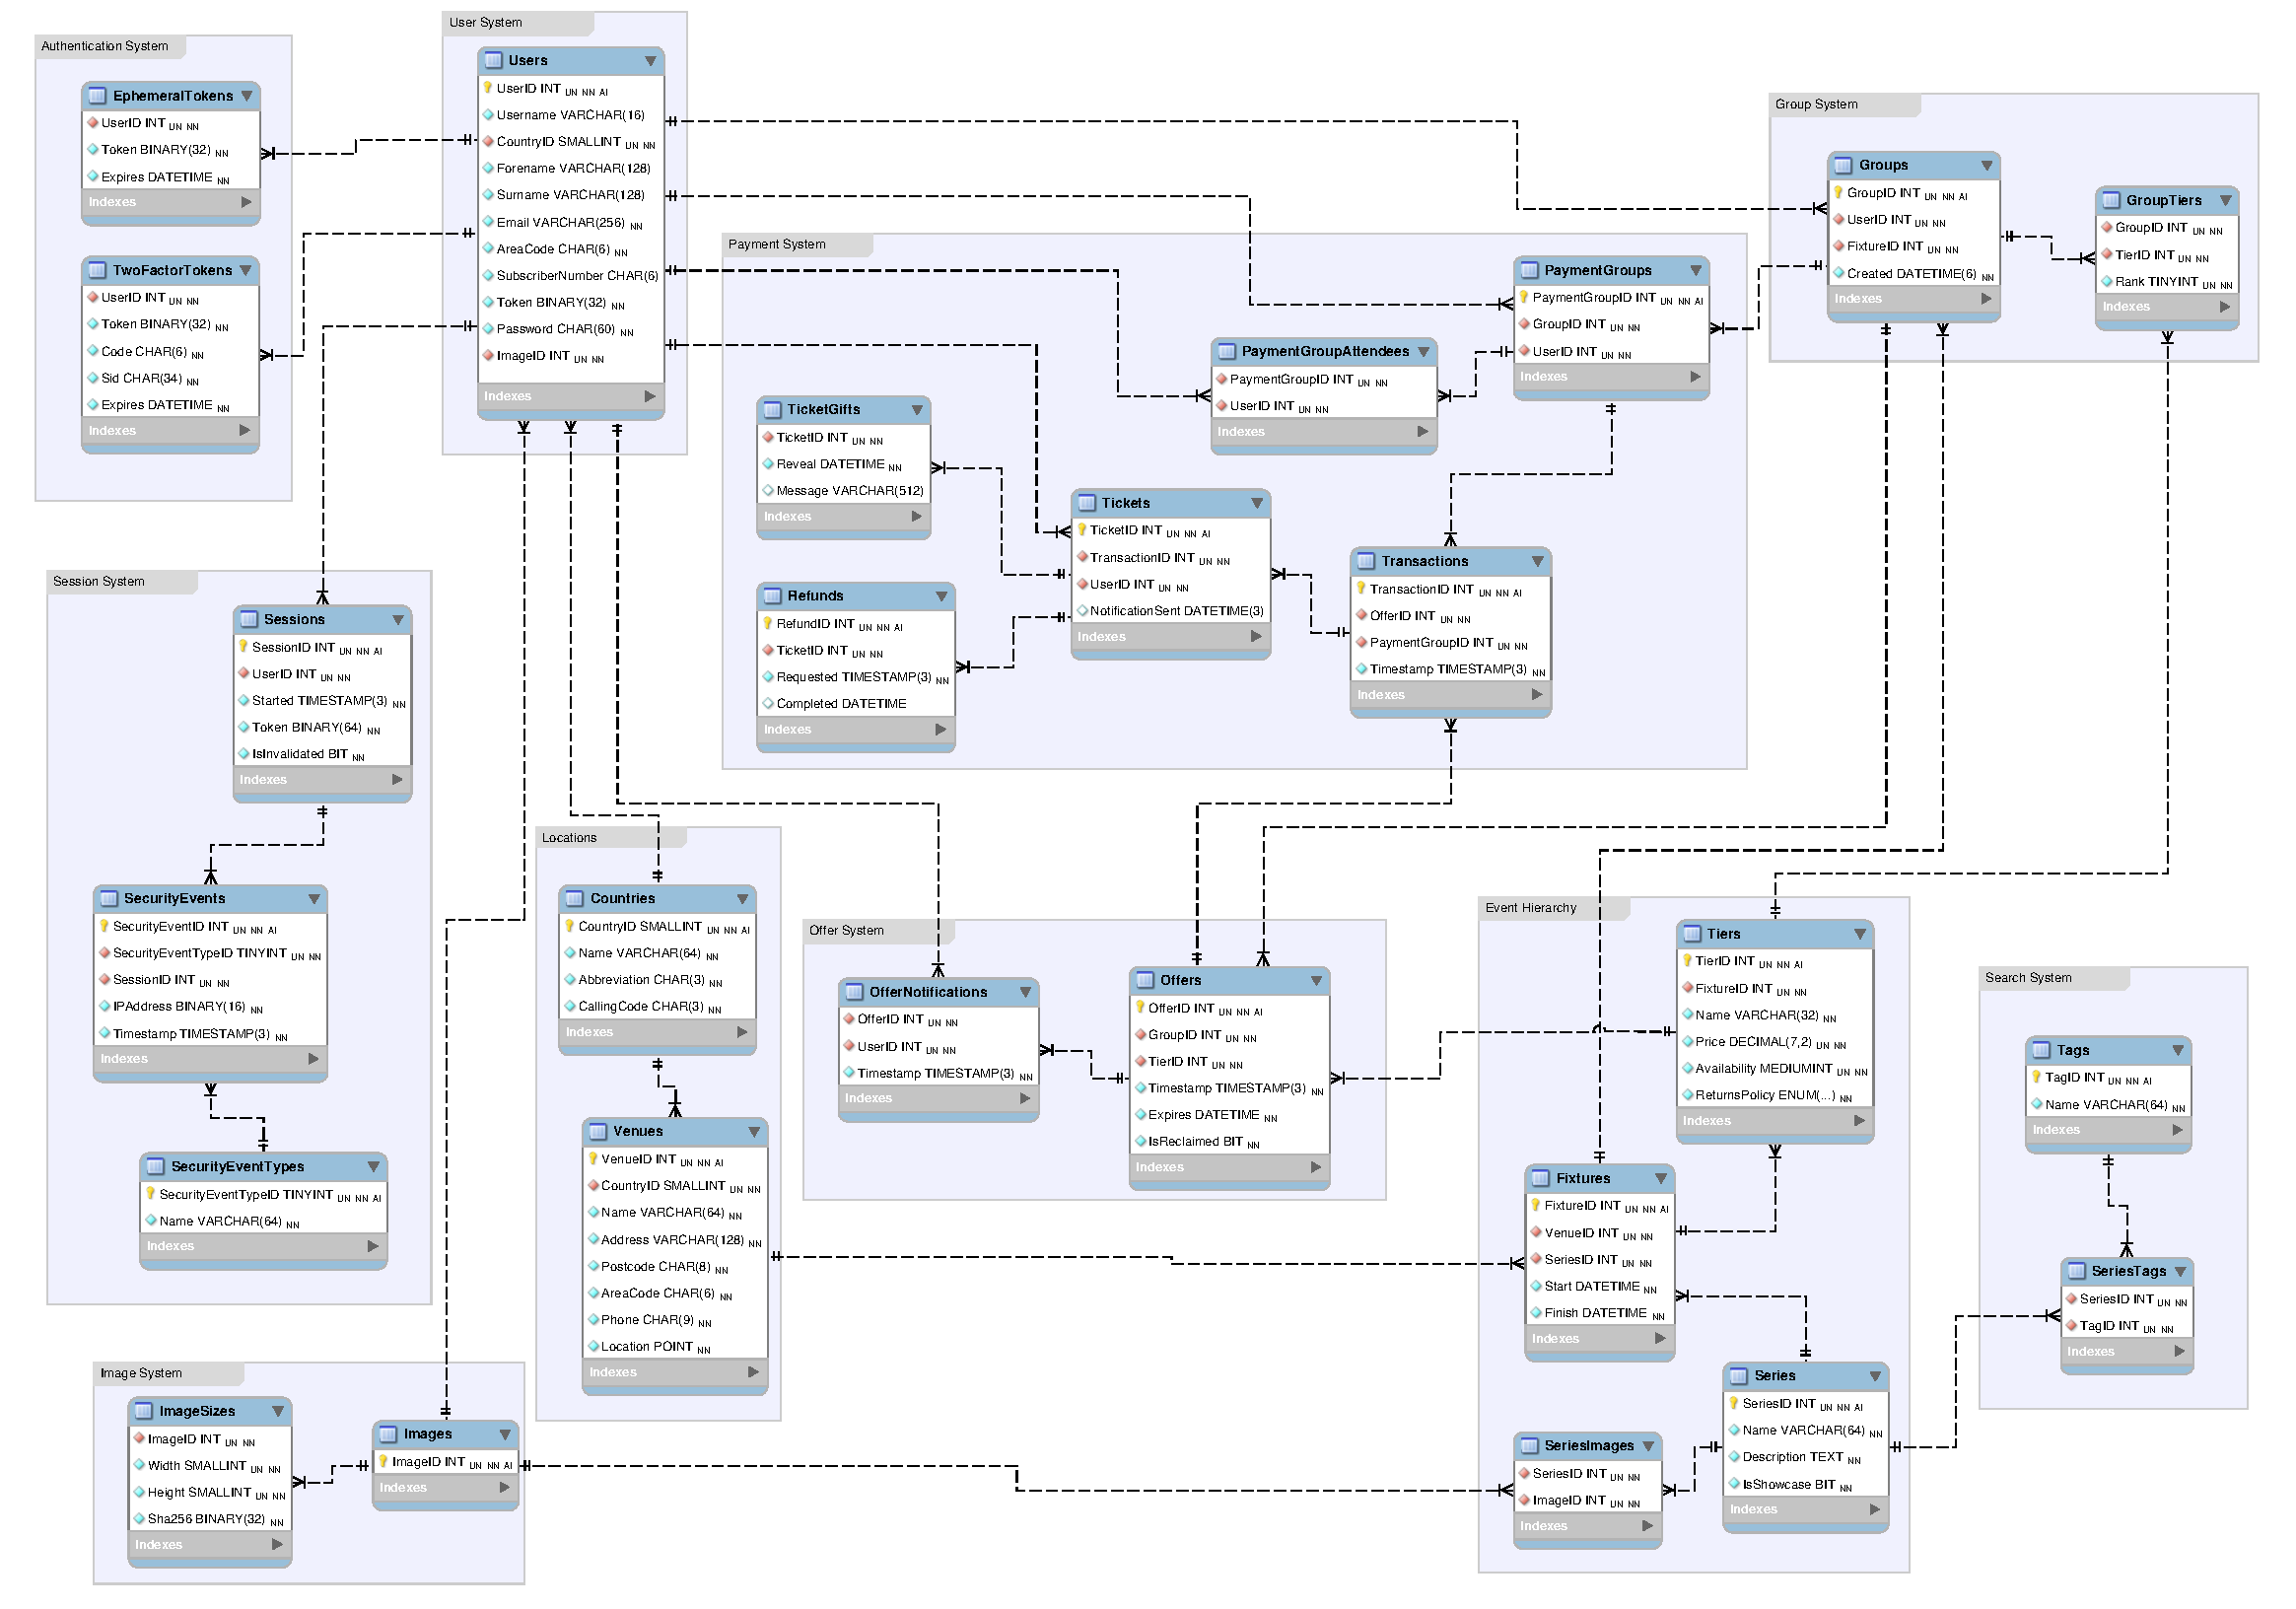
\includegraphics[width=1.1\linewidth]{img/database.pdf}
        }
        \caption{Equaliser database schema}
        \label{fig:database}
    \end{figure}
\end{landscape}

From a performance perspective, there are hot (i.e. active) and cold tables within the database. These generally separate into those touched by customers and those touched by organisers respectively. Fortunately, with the exception of the orders table and group hierarchy, the most active tables are written to by a background process, meaning users will not be exposed to any slowness in writing to these tables. The orders table and group hierarchy are write only, so it would be safe to cache their contents indefinitely should performance not be sufficient. The structure itself is favourable to sharding, as there is no cross-access of hot rows.

Regarding the barrier client used by venue staff, depending on the venue size, it is possible for there to be contention when retrieving lots of photos and user information. It would be trivial to export the orders for a single event, along with the photos of everyone in attendance, and run the barrier system on this. Assuming a sold out 90,000 seat venue and 100KiB per profile photo, such a dataset would occupy 9.21GiB of memory. Not only would this speed up retrieval time, but it would remove the possibility of internet connectivity issues. For those events not large enough to warrant dedicated hardware, or with a reliable internet connection, this information could be located in a data-centre near the venue to reduce latency.

\subsection{Verticles}

Verticles can be thought of as individual applications that can communicate cheaply. I knew the system would need background processes for several tasks, and each naturally mapped into a verticle. In total, Equaliser uses 6:

\begin{description}
    \item[RestVerticle] Handles API requests; the only public-facing verticle. 
    \item[OfferIssueVerticle] Periodically assigns tickets in the secondary pool to groups in the waiting list. If deemed necessary, this will also process pending refunds to free up more tickets.
    \item[OfferReclaimVerticle] Periodically scans for expired unclaimed offers and adds the tickets behind them to the secondary pool.
    \item[PrimaryPoolVerticle] Maintains a hash map of tiers to available tickets. The counts represent new tickets that have not been sold.
    \item[SecondaryPoolVerticle] Similar to \code{PrimaryPoolVerticle}, this does the book keeping for returned tickets.
    \item[TicketNotificationVerticle] Periodically scans for issued tickets, sending SMS notifications to their owners using Twilio.
\end{description}

Vert.x allows scaling each of these up individually with no increase in complexity or latency, making them very suitable for Equaliser's desired level of performance. For example, as Twilio's API typically takes 300-400ms to return a response, it will be essential to have many instances of this verticle running to keep up with tickets being issued.

\subsection{Authentication} \label{tech_design_api_authentication}

While some endpoints are public, such as those used to list event details, others are private, including those for retrieving and creating orders. In a conventional web application, cookies would be used to allow stateful handling of requests, however in the context of an API, this is notoriously bad design. I considered OAuth, however it is primarily designed to allow third party applications to access data, and so far, none of these existed. In the interest of simplicity, which I regard as being the one and only pillar of maintainability, Equaliser instead uses a 64 byte session token, which is returned on successful authentication. It is passed in the HTTP \code{Authorization} header of all requests requiring the user to be logged in. In the backend, this token is transparently validated, and the user's session object becomes an implicit input to those endpoints, as if it were a normal \code{GET} parameter or \code{POST} field.

To authenticate, the client sends a \code{POST} request to \code{\path{/auth/first}} with \code{username} and \code{password} fields. This is analogous to the login form on most websites. If these credentials match an account, the backend generates a 6-digit code and sends it within an SMS to the phone number associated with that account using Twilio's SMS service. An example of a received message is shown in Figure \ref{img:2fa_code}. This message will display with a heading of ``Equaliser'' rather than a phone number, as Alphanumeric Sender ID \footnote{\url{https://support.twilio.com/hc/en-us/articles/223181348-Getting-started-with-Alphanumeric-Sender-ID}} is in use. The backend also generates 32 bytes of random data, and stores it with the code in the \code{TwoFactorTokens} table. This random data is then returned to the user.

\begin{figure}[!htbp]
    \centering
    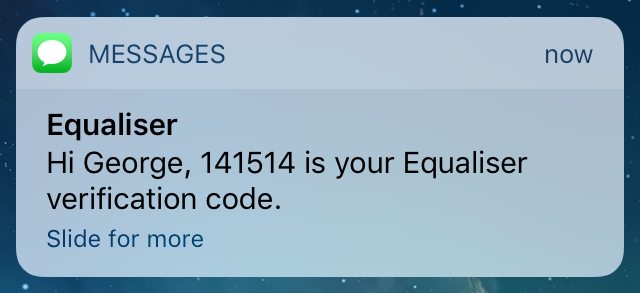
\includegraphics[width=.6\linewidth]{img/2fa_code.png}
    \caption{Two-factor authentication code received on an iPhone}
    \label{img:2fa_code}
\end{figure}

To complete authentication, the client must now send a \code{POST} request to \code{\path{/auth/second}} containing the 6-digit code and corresponding random data. This ties the authentication attempt to both the phone and the prior login details. If the token and code match to a row, authentication succeeds, and an eternal, but revocable session token is generated and returned, along with the \code{User} object. All authentication artefacts are deleted, so they cannot be used in a replay attack. Figure \ref{img:2fa_interaction} shows this entire process.

\begin{figure}[!htbp]
    \centering
    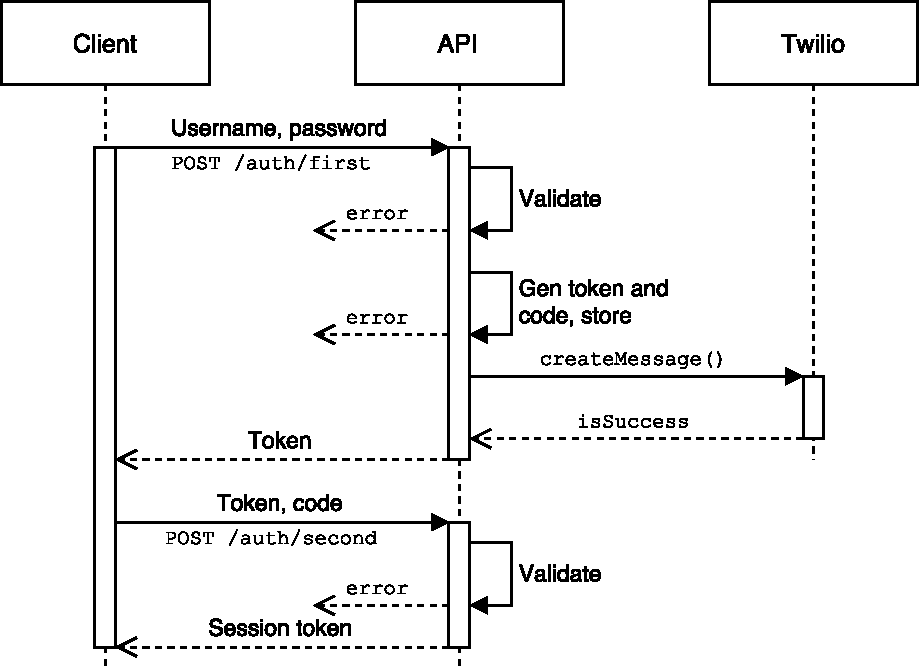
\includegraphics[width=.8\linewidth]{img/2fa_interaction.pdf}
    \caption{Two-factor flow interaction diagram}
    \label{img:2fa_interaction}
\end{figure}

\section{Website}

Along with the mobile app, the website is a second consumer of the REST service. It exists both to demonstrate the generality of the API, and originally as somewhat of a fall back in case the mobile app turned out to be too great an undertaking. Fortunately, that turned out not to be the case, and I was able to implement several features exploiting both clients, for example the co-operative authentication, which will be discussed in due course.

As this component was essentially a user interface, it contained very little back-end complexity. In order to avoid spending any more time on it than necessary, I used the Django Python library, which makes it very easy to quickly set up MVC web applications.

\subsection{State}

There is no reason for the website to maintain any state whatsoever; this is the function of the API's database. If I had known a front-end framework like AngularJS, I would have used this without a second thought, as the website back-end could be entirely static, with all computation happening between end-user browsers and the API. Unfortunately, this component highlighted a gap in my knowledge. Given more time, I would definitely like to spend more time re-implementing the web app in a more suitable language. Django itself requires a database, however it abstracts away the specific one in use. In the interests of time, I used a local SQLite database.

\subsection{Design}

I started by mocking up a static version of each page using only HTML and CSS, then added in JavaScript where necessary, for example to allow adding users to an order and toggling whether their ticket is gifted. I took inspiration from many existing ticket distributors, particularly DICE, however Equaliser's design is unique, and built from scratch. The front page is a showcase of series and fixtures available for booking. A mock-up can be seen in Figure \ref{img:showcase}. The large image behind the ``Equaliser'' text is chosen at random from a list of eligible series that lend themselves to such a display. Each thumbnail below is a series within that category. These rows scroll left and right to show more.

\begin{figure}[!htbp]
    \centering
    \includegraphics[width=1\linewidth]{img/showcase.png}
    \caption{The website homepage}
    \label{img:showcase}
\end{figure}

Clicking a series will take the user to its page, an example of which is shown in Figure \ref{img:series}. I was surprised to find that many ticket distributors include little description of events; users are simply trusted to know what to buy, with almost no marketing. Equaliser allows event organisers to select a background image and optionally include a description. Beneath these are fixtures. The series in the example has three, each showing available tiers and prices. Orange ``Wait'' buttons are displays when a particular tier has sold out, while green ``Buy'' buttons are shown for those with seats left. Of course, there is no guarantee that availability will not change between a button being rendered and clicked.

\begin{figure}[!htbp]
    \centering
    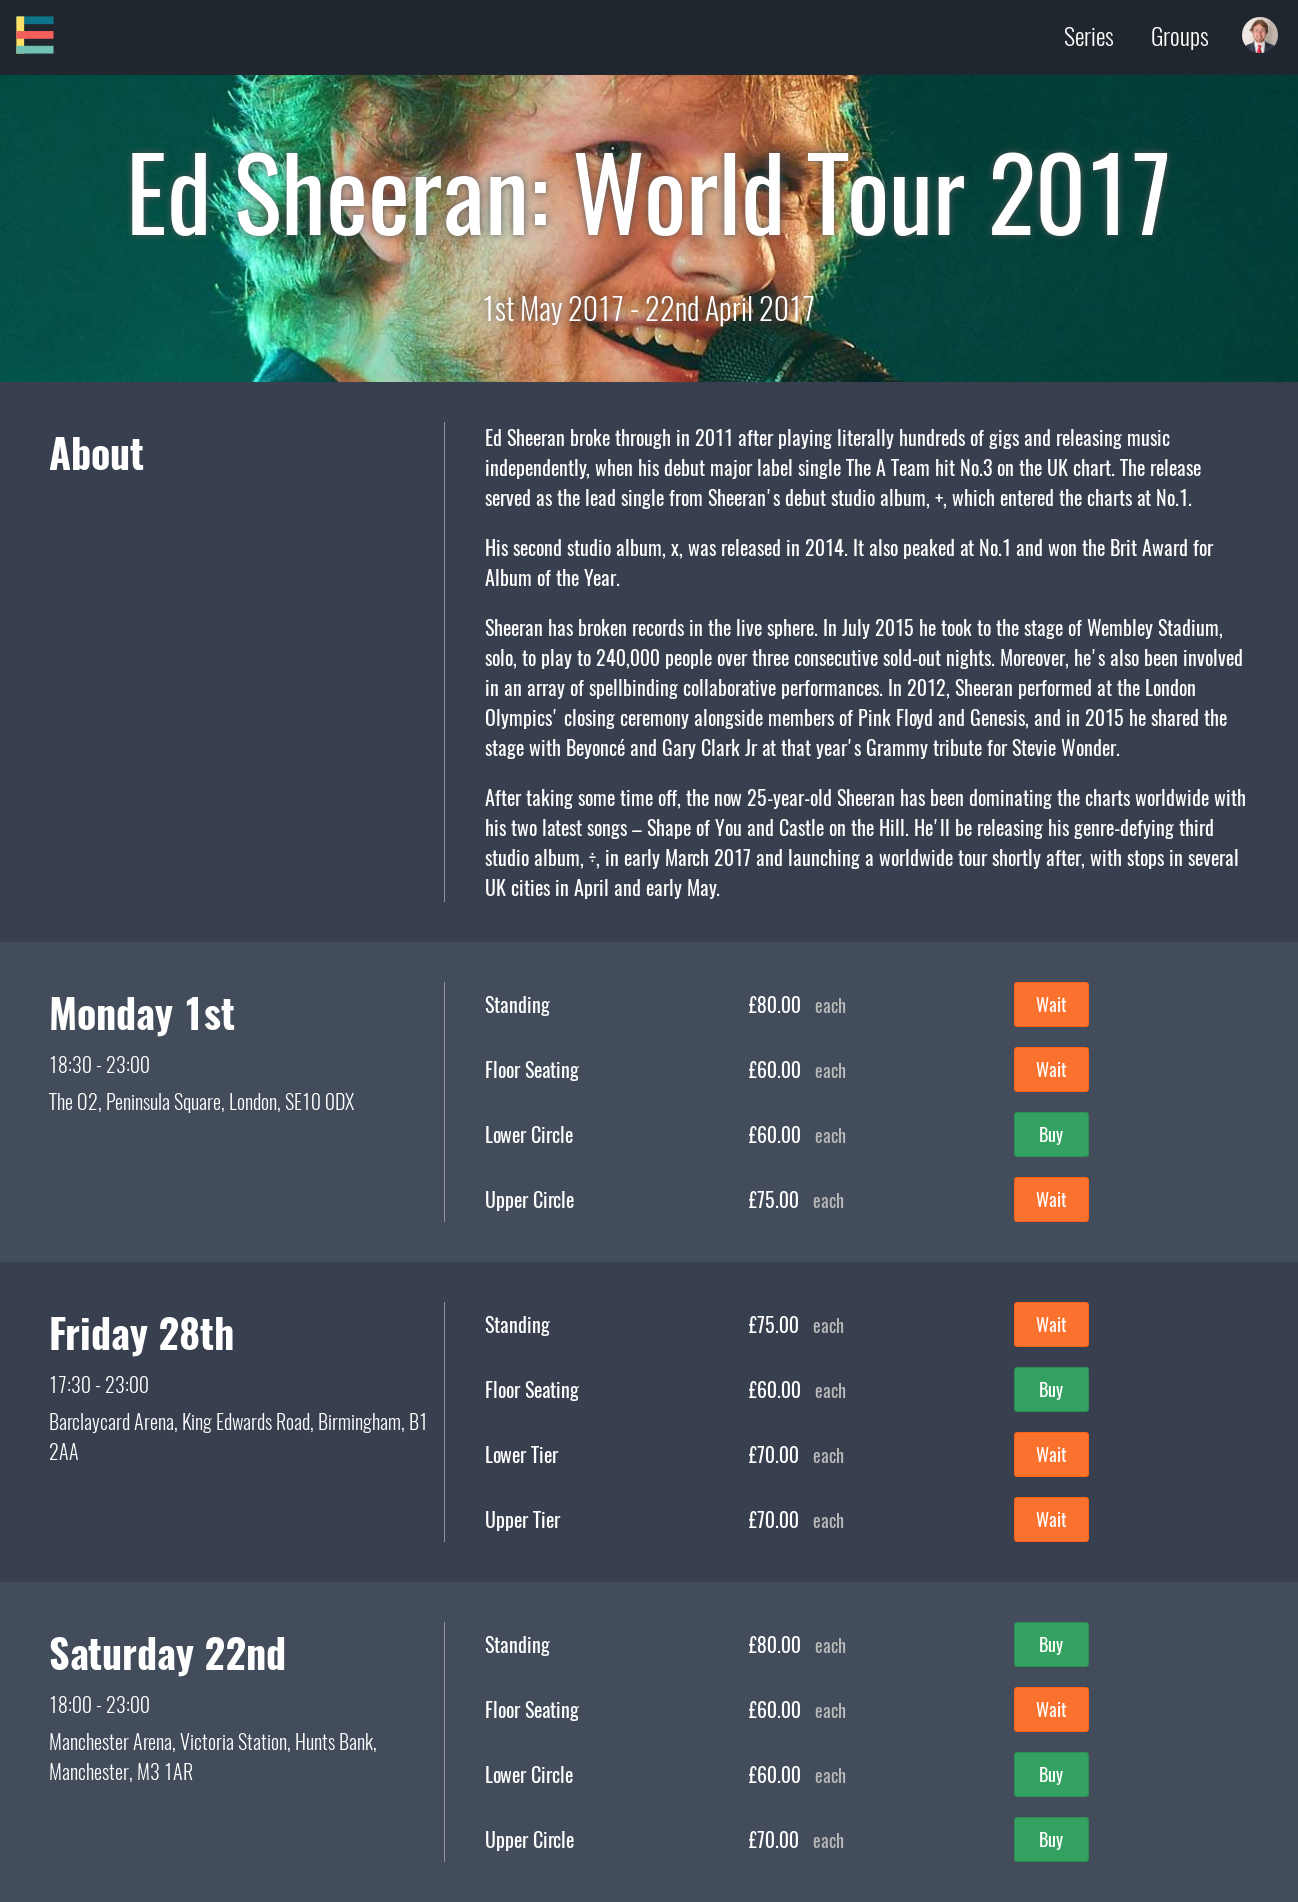
\includegraphics[width=1\linewidth]{img/series.png}
    \caption{A series page}
    \label{img:series}
\end{figure}

\subsection{Security}

The website itself delegates all security to the underlying API system, which assumes all clients are potentially malicious, and limits the website in the same way it would limit a mobile phone. The website does however give users insight into how their account it being used via a security event log, shown in Figure \ref{img:account}.

\begin{figure}[!htbp]
    \centering
    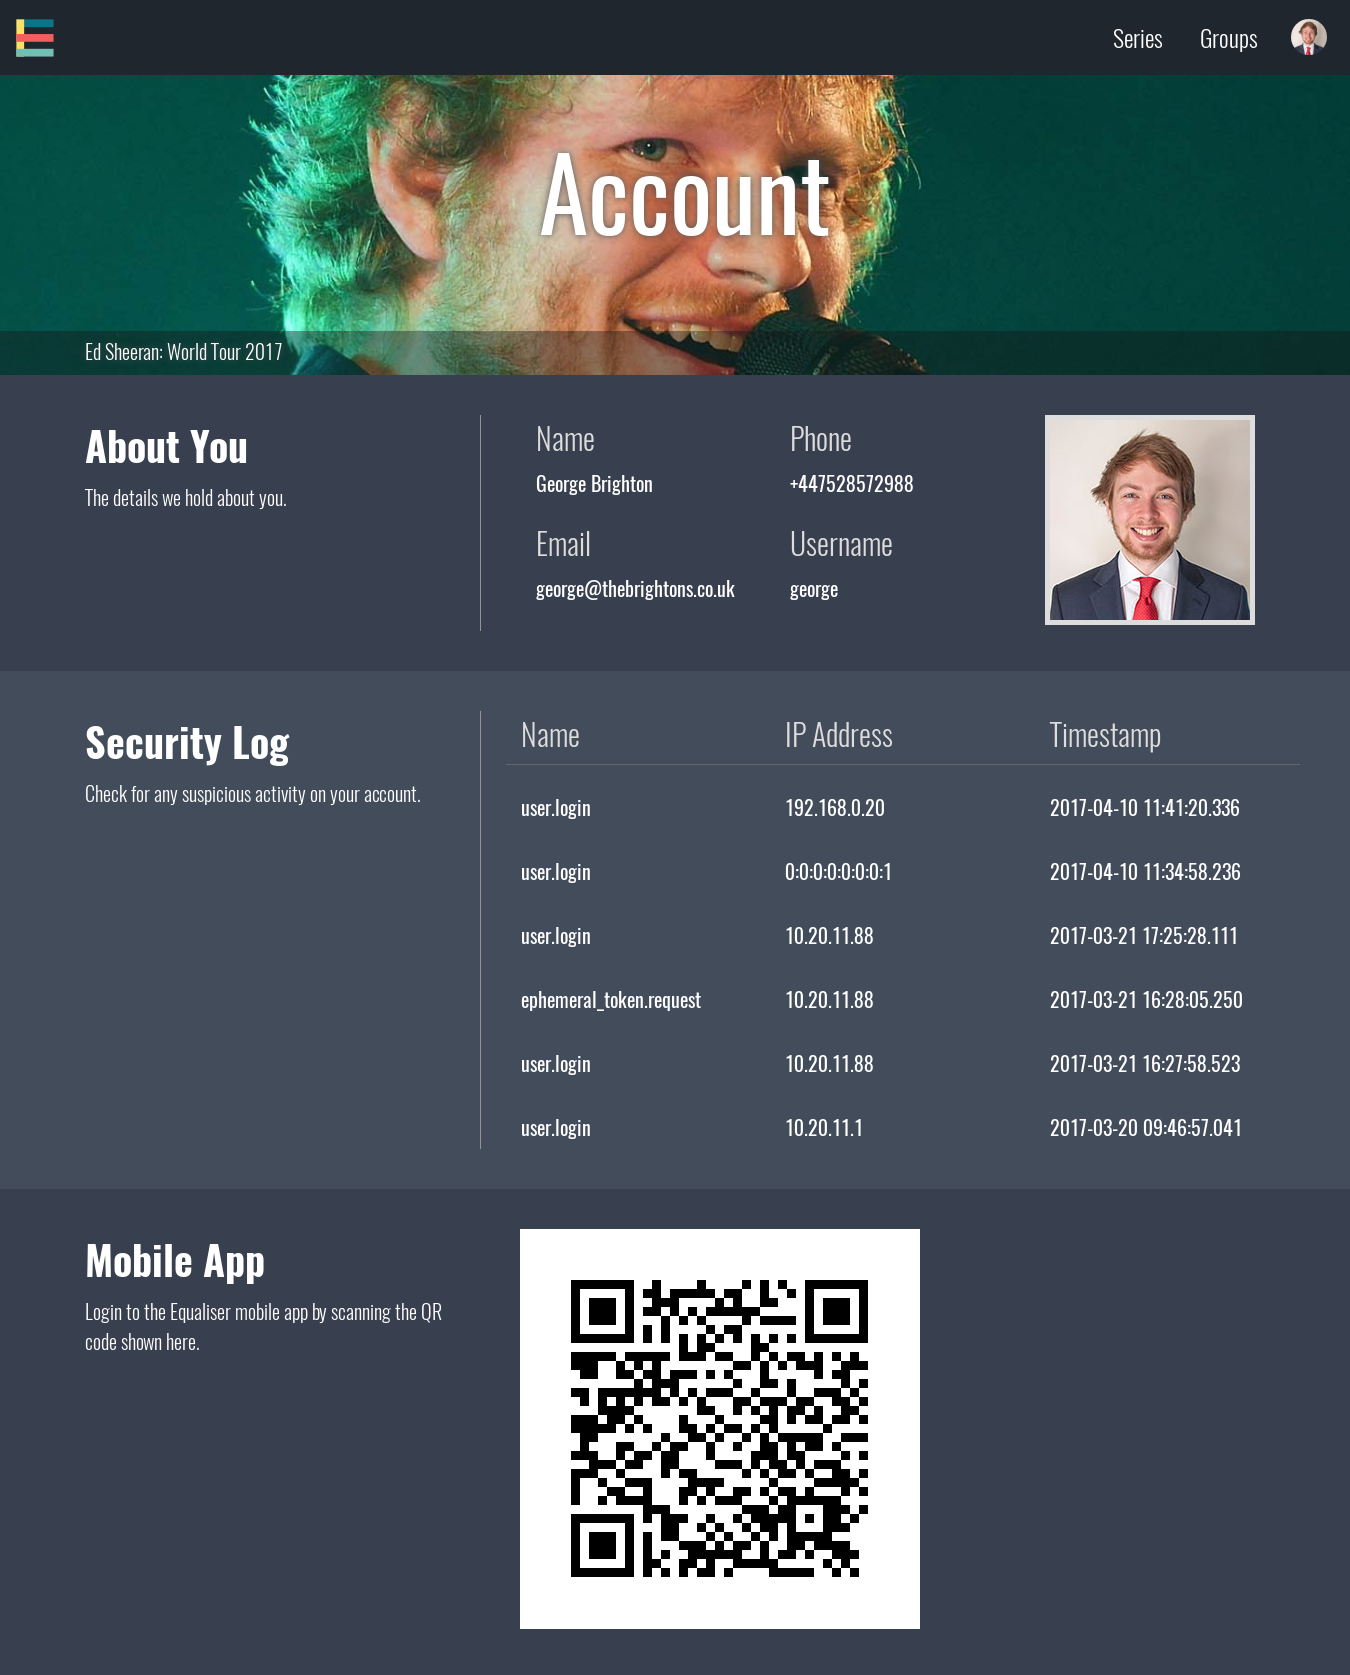
\includegraphics[width=1\linewidth]{img/account.png}
    \caption{The account page}
    \label{img:account}
\end{figure}

When notable events are triggered, such as user logins and ephemeral token generations, the backend records these in a dedicated set of tables. These can be seen on the left hand side of Figure \ref{fig:database}. Although not implemented, it would be easy to extend this to allow users to flag suspicious activity, revoke authentication tokens and so on.

\section{Mobile App}

% TODO get Helen to check

Prior to this project, I had no experience with mobile development. As an iPhone user, I considered targeting iOS, however the requirement for Xcode, which in turn requires MacOS meant this was off the cards, even before the additional hurdle of not knowing Swift or Objective-C. Android was the clear solution in order to be productive and solve the interesting problems, otherwise Equaliser may have dissolved into learning another language.

\subsection{Design}

The mobile app implements equivalent functionality to the website. Once logged in, it allows the user to browse events, shown in Figure \ref{img:app_browse}. Most importantly, everything visible in the app is using the same API as the website. The website may choose larger versions of images to suit the generally larger screen sizes of, however this is a client-side choice.

Tapping a series will display its details, shown in Figure \ref{img:app_series}. Scrolling down to below the description will show fixtures available for booking, demonstrated in Figure \ref{img:app_fixtures}.

\begin{figure}[!htbp]
  \centering
  \hspace{0.05\textwidth}
  \begin{minipage}[b]{0.4\textwidth}
    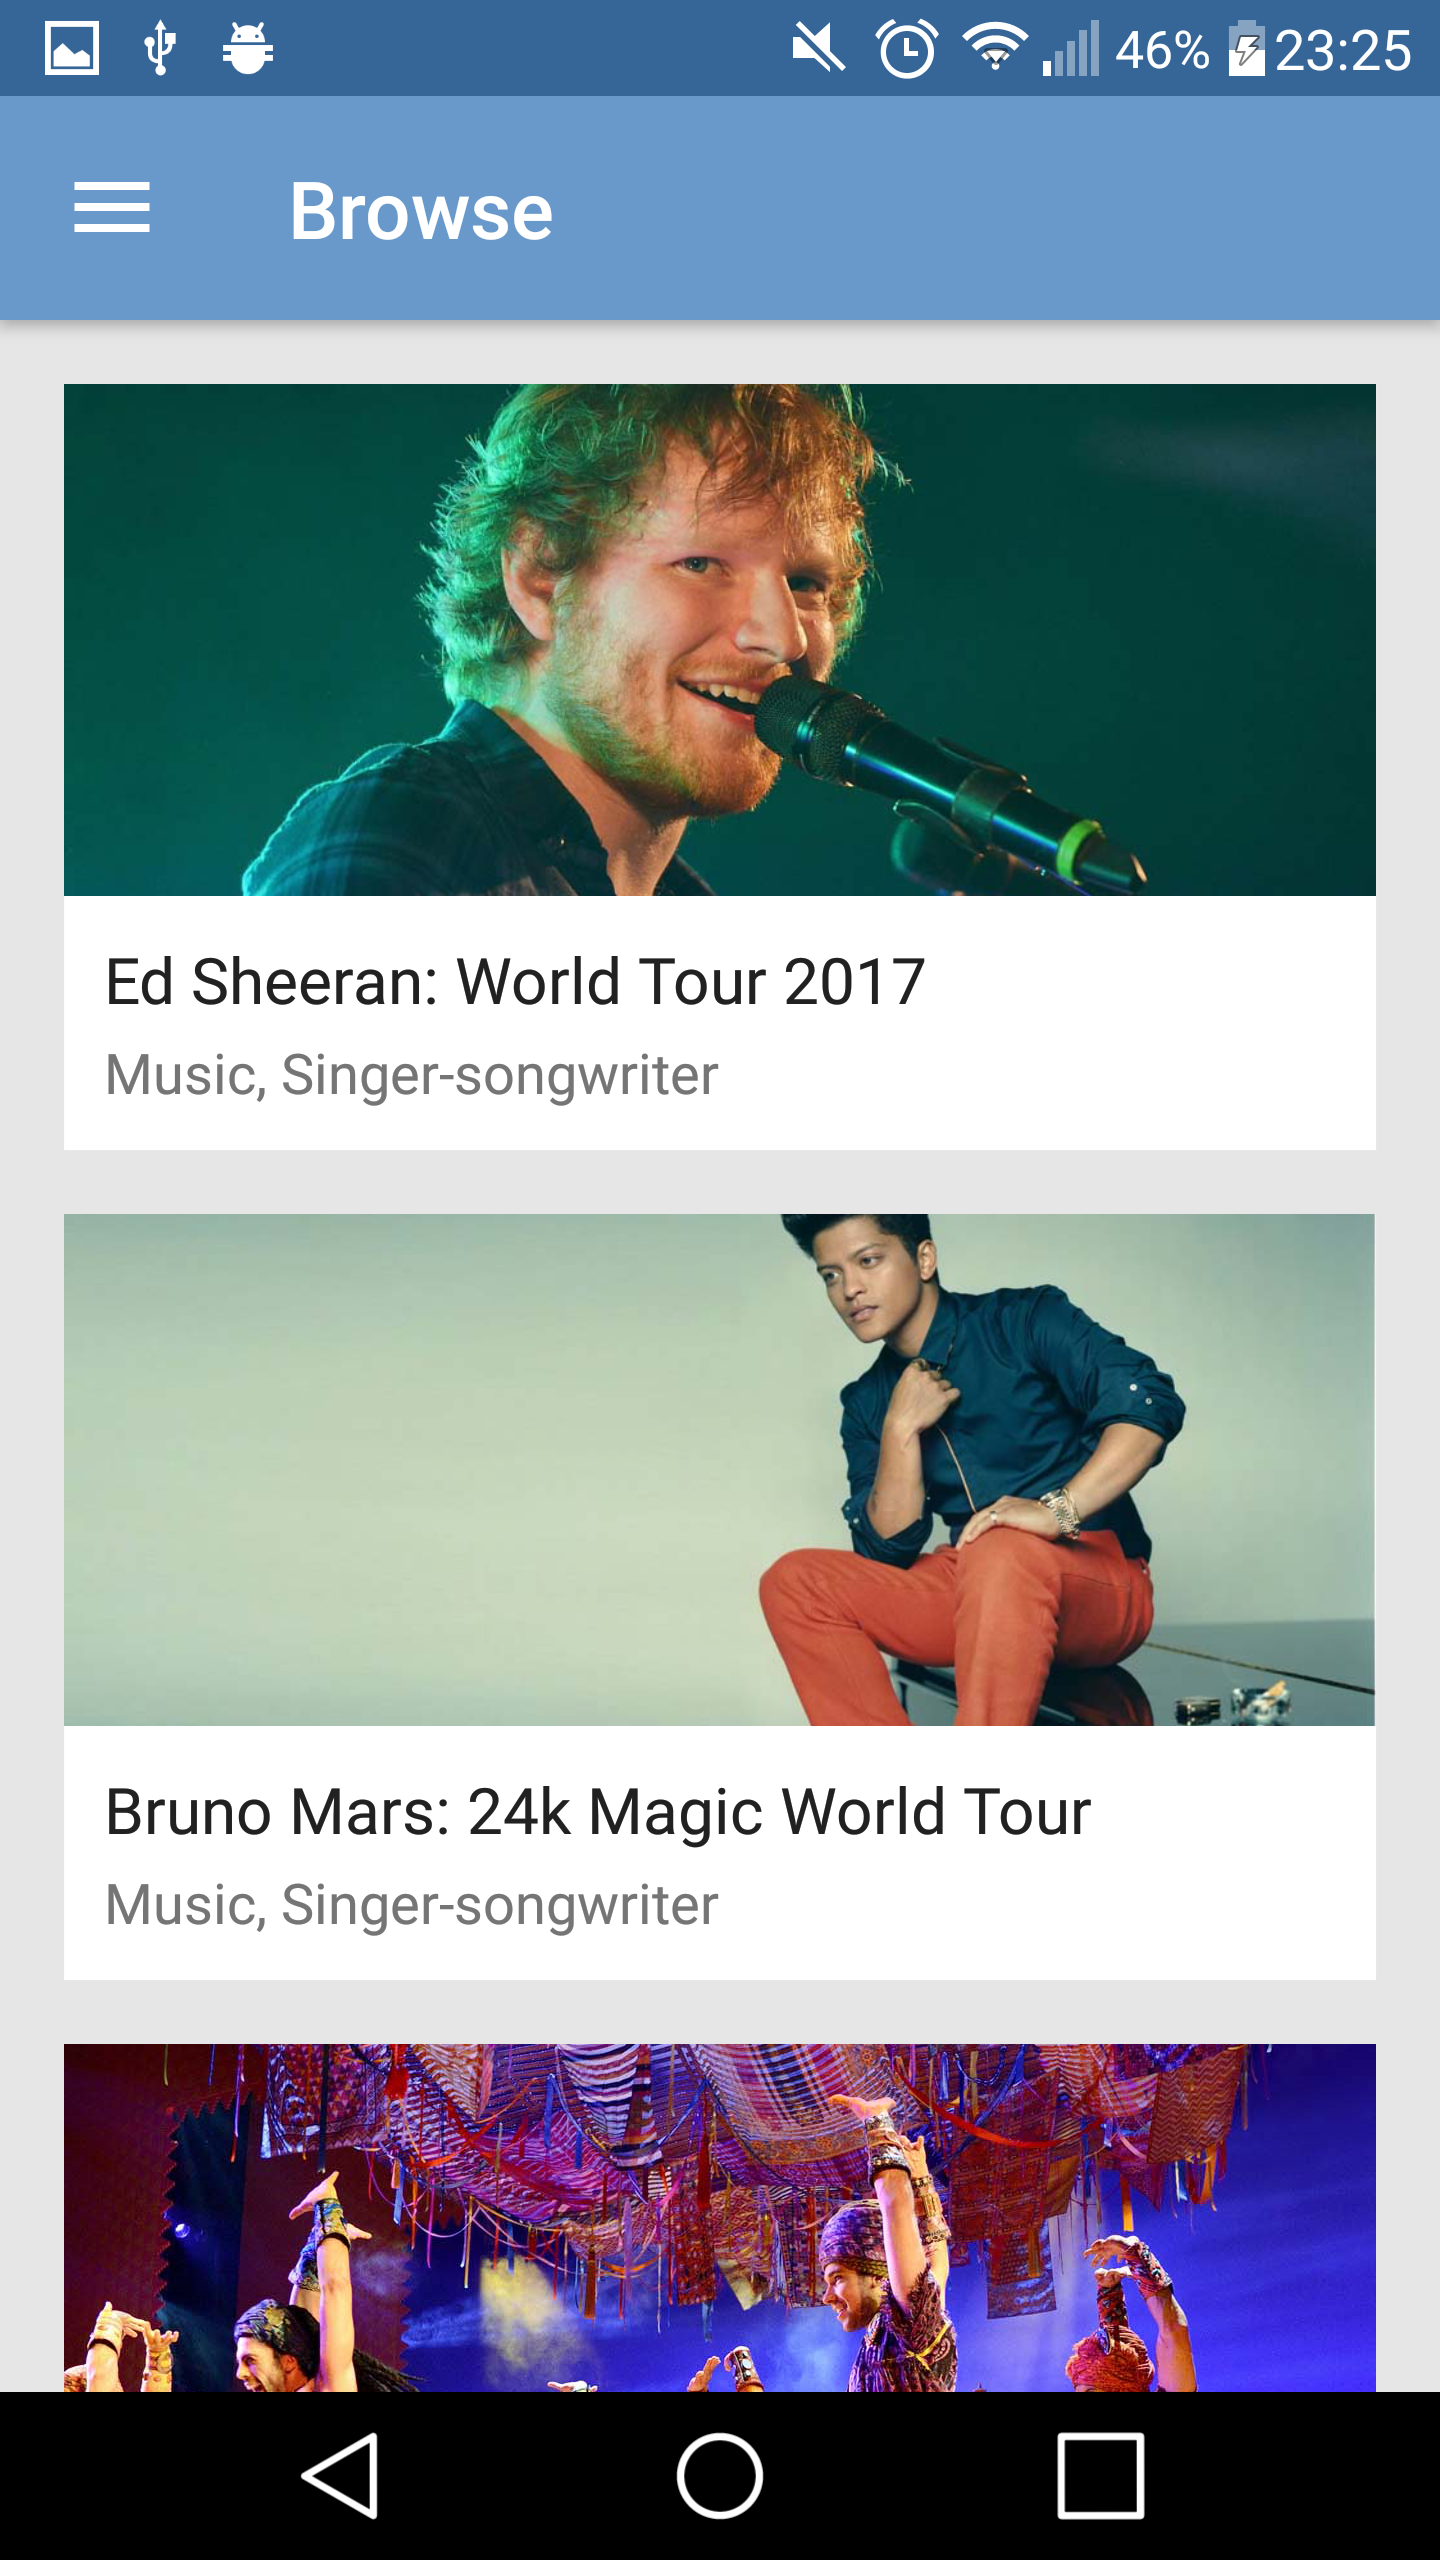
\includegraphics[width=\textwidth]{img/app_browse.png}
    \caption{The home screen}
    \label{img:app_browse}
  \end{minipage}
  \hfill
  \begin{minipage}[b]{0.4\textwidth}
    
\includegraphics[width=\textwidth]{img/app_series.png}
    \caption{The series screen}
    \label{img:app_series}
  \end{minipage}
  \hspace{0.05\textwidth}
\end{figure}

\begin{figure}[!htbp]
    \centering
    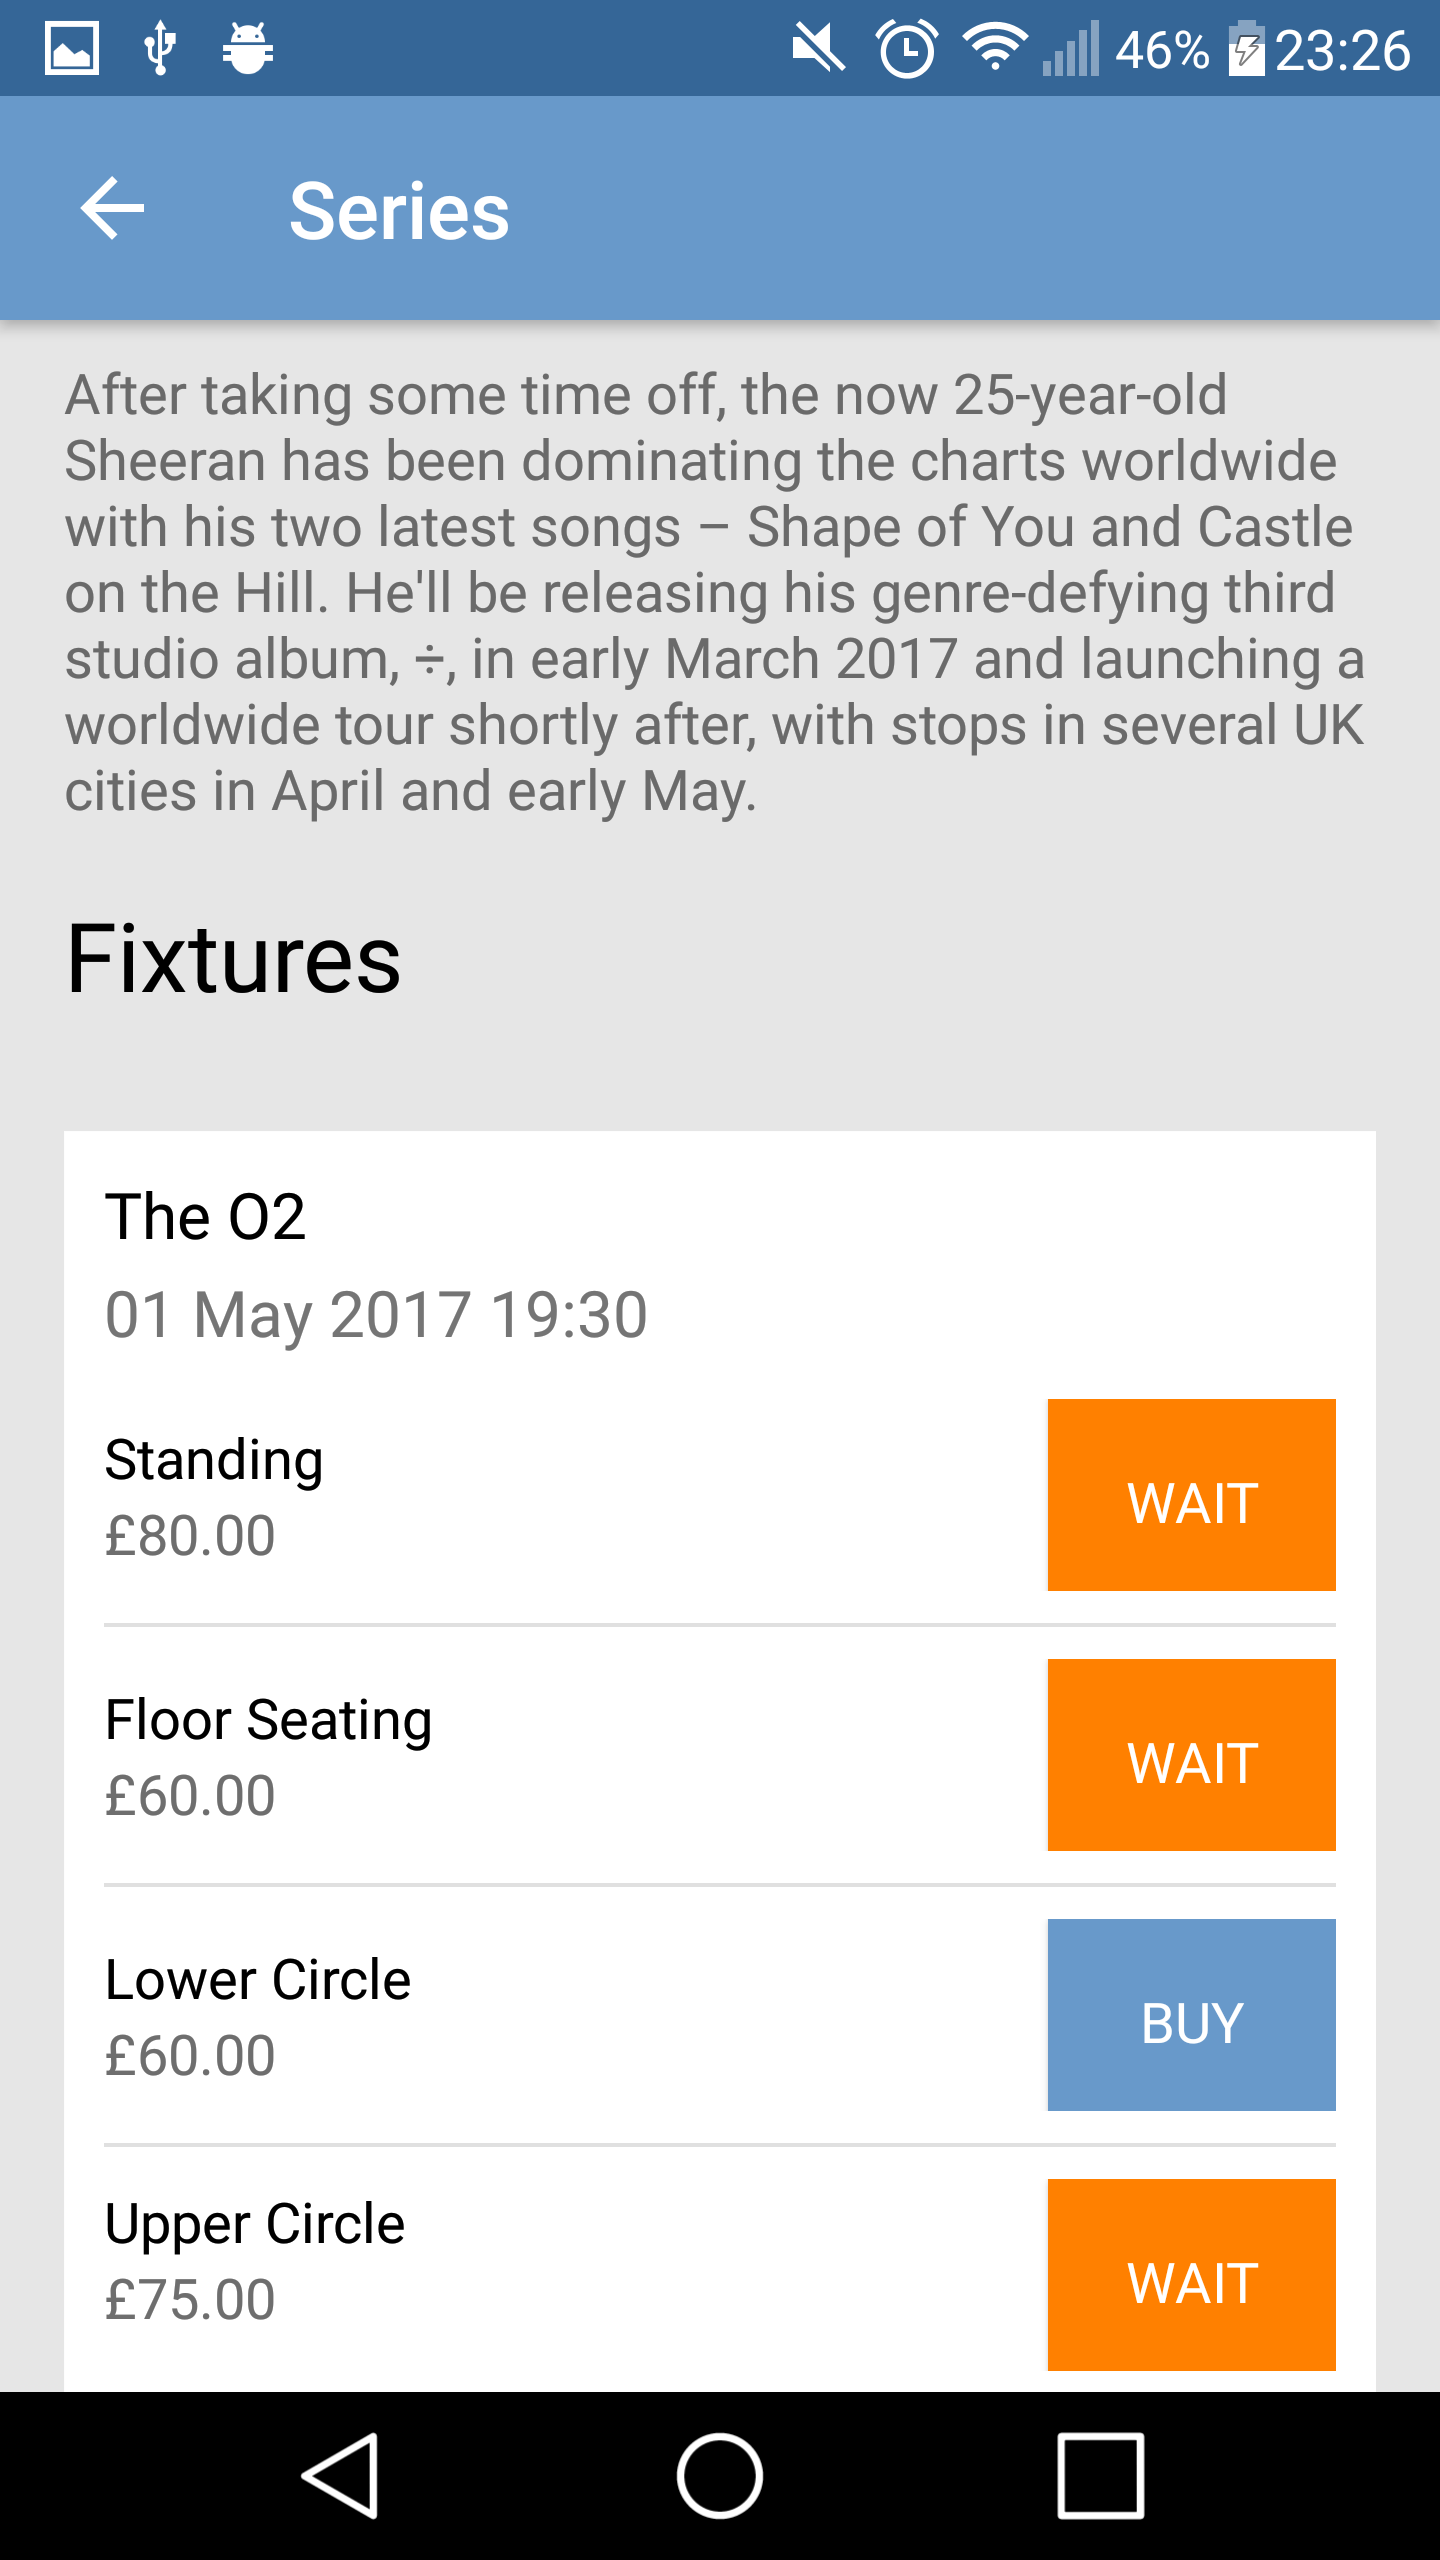
\includegraphics[width=.5\linewidth]{img/app_fixtures.png}
    \caption{The bottom of the series screen, showing fixtures available for booking}
    \label{img:app_fixtures}
\end{figure}

\subsection{Co-operative Authentication}

Rather than allow users to sign in on their phones with a simple username and password, I wanted to implement something as close to a second factor as possible. I had been impressed by WhatsApp's method of authenticating the web client using the mobile client, and decided to do this in reverse for Equaliser. This exploits the fact that users have already passed through the authentication flow once, so we can be sure of their identity. Login is also reduced to scanning a code, making it quick and simple.

An authenticated client begins the process by sending a \code{GET} request to \code{\path{/auth/ephemeral}}. As the user has provided an \code{Authorization} header, they can be securely identified from this alone. The backend generates 32 random bytes, stores them in the database, and returns the data as a QR code, shown as it appears on the website in Figure \ref{fig:ephemeral_qr_code}.

\begin{figure}[!htbp]
    \centering
    
\includegraphics[width=1\linewidth]{img/ephemeral_qr_code.png}
    \caption{Ephemeral token QR code, representing 32 bytes of random data}
    \label{fig:ephemeral_qr_code}
\end{figure}

The user then starts the Equaliser app, which in its initial state will resemble Figure \ref{fig:app_initial}. They can tap the scan button, and point it at the QR code image, as demonstrated in Figure \ref{fig:app_qr_scan}. As can be seen from the turquoise text in this image, the QR code is an arbitrary sequence of hex digits. They have no meaning; it is simply a random value associated with a user, that is sufficiently long enough to be unguessable for practical purposes.

\begin{figure}[!htbp]
  \centering
  \hspace{0.05\textwidth}
  \begin{minipage}[b]{0.4\textwidth}
    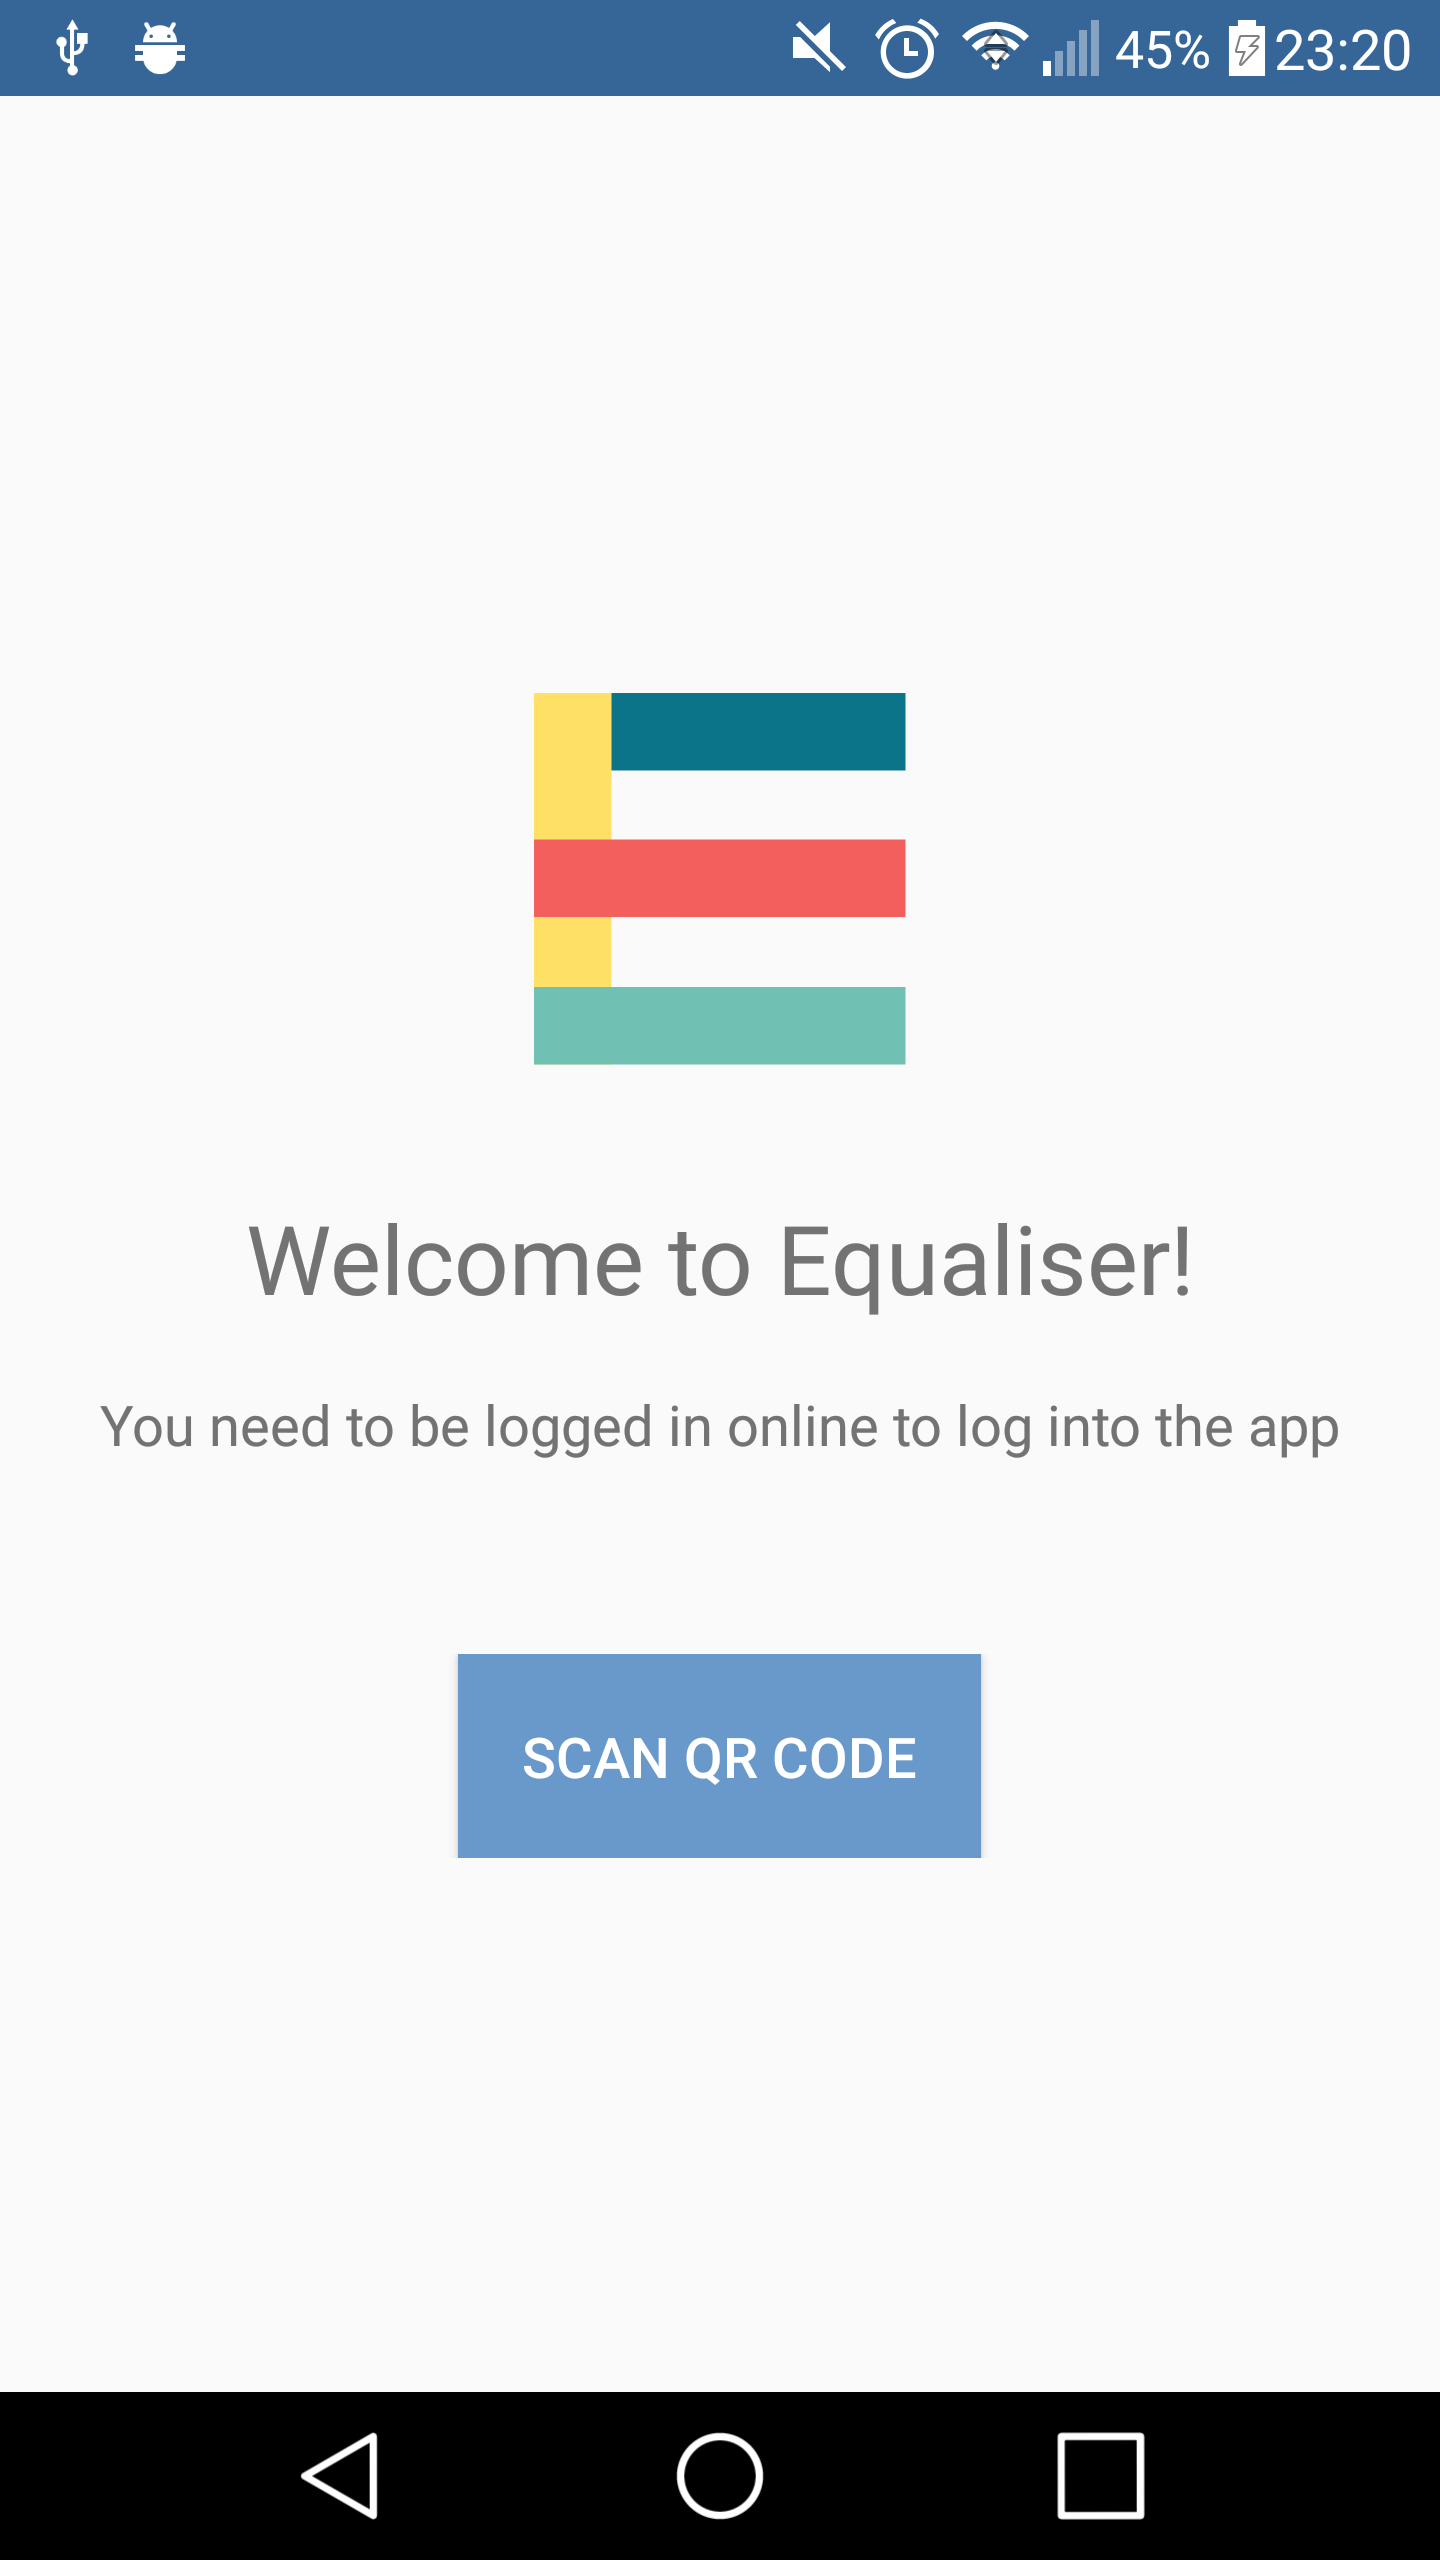
\includegraphics[width=\textwidth]{img/app_initial.png}
    \caption{The mobile app in its initial, or logged-out state}
    \label{fig:app_initial}
  \end{minipage}
  \hfill
  \begin{minipage}[b]{0.4\textwidth}
    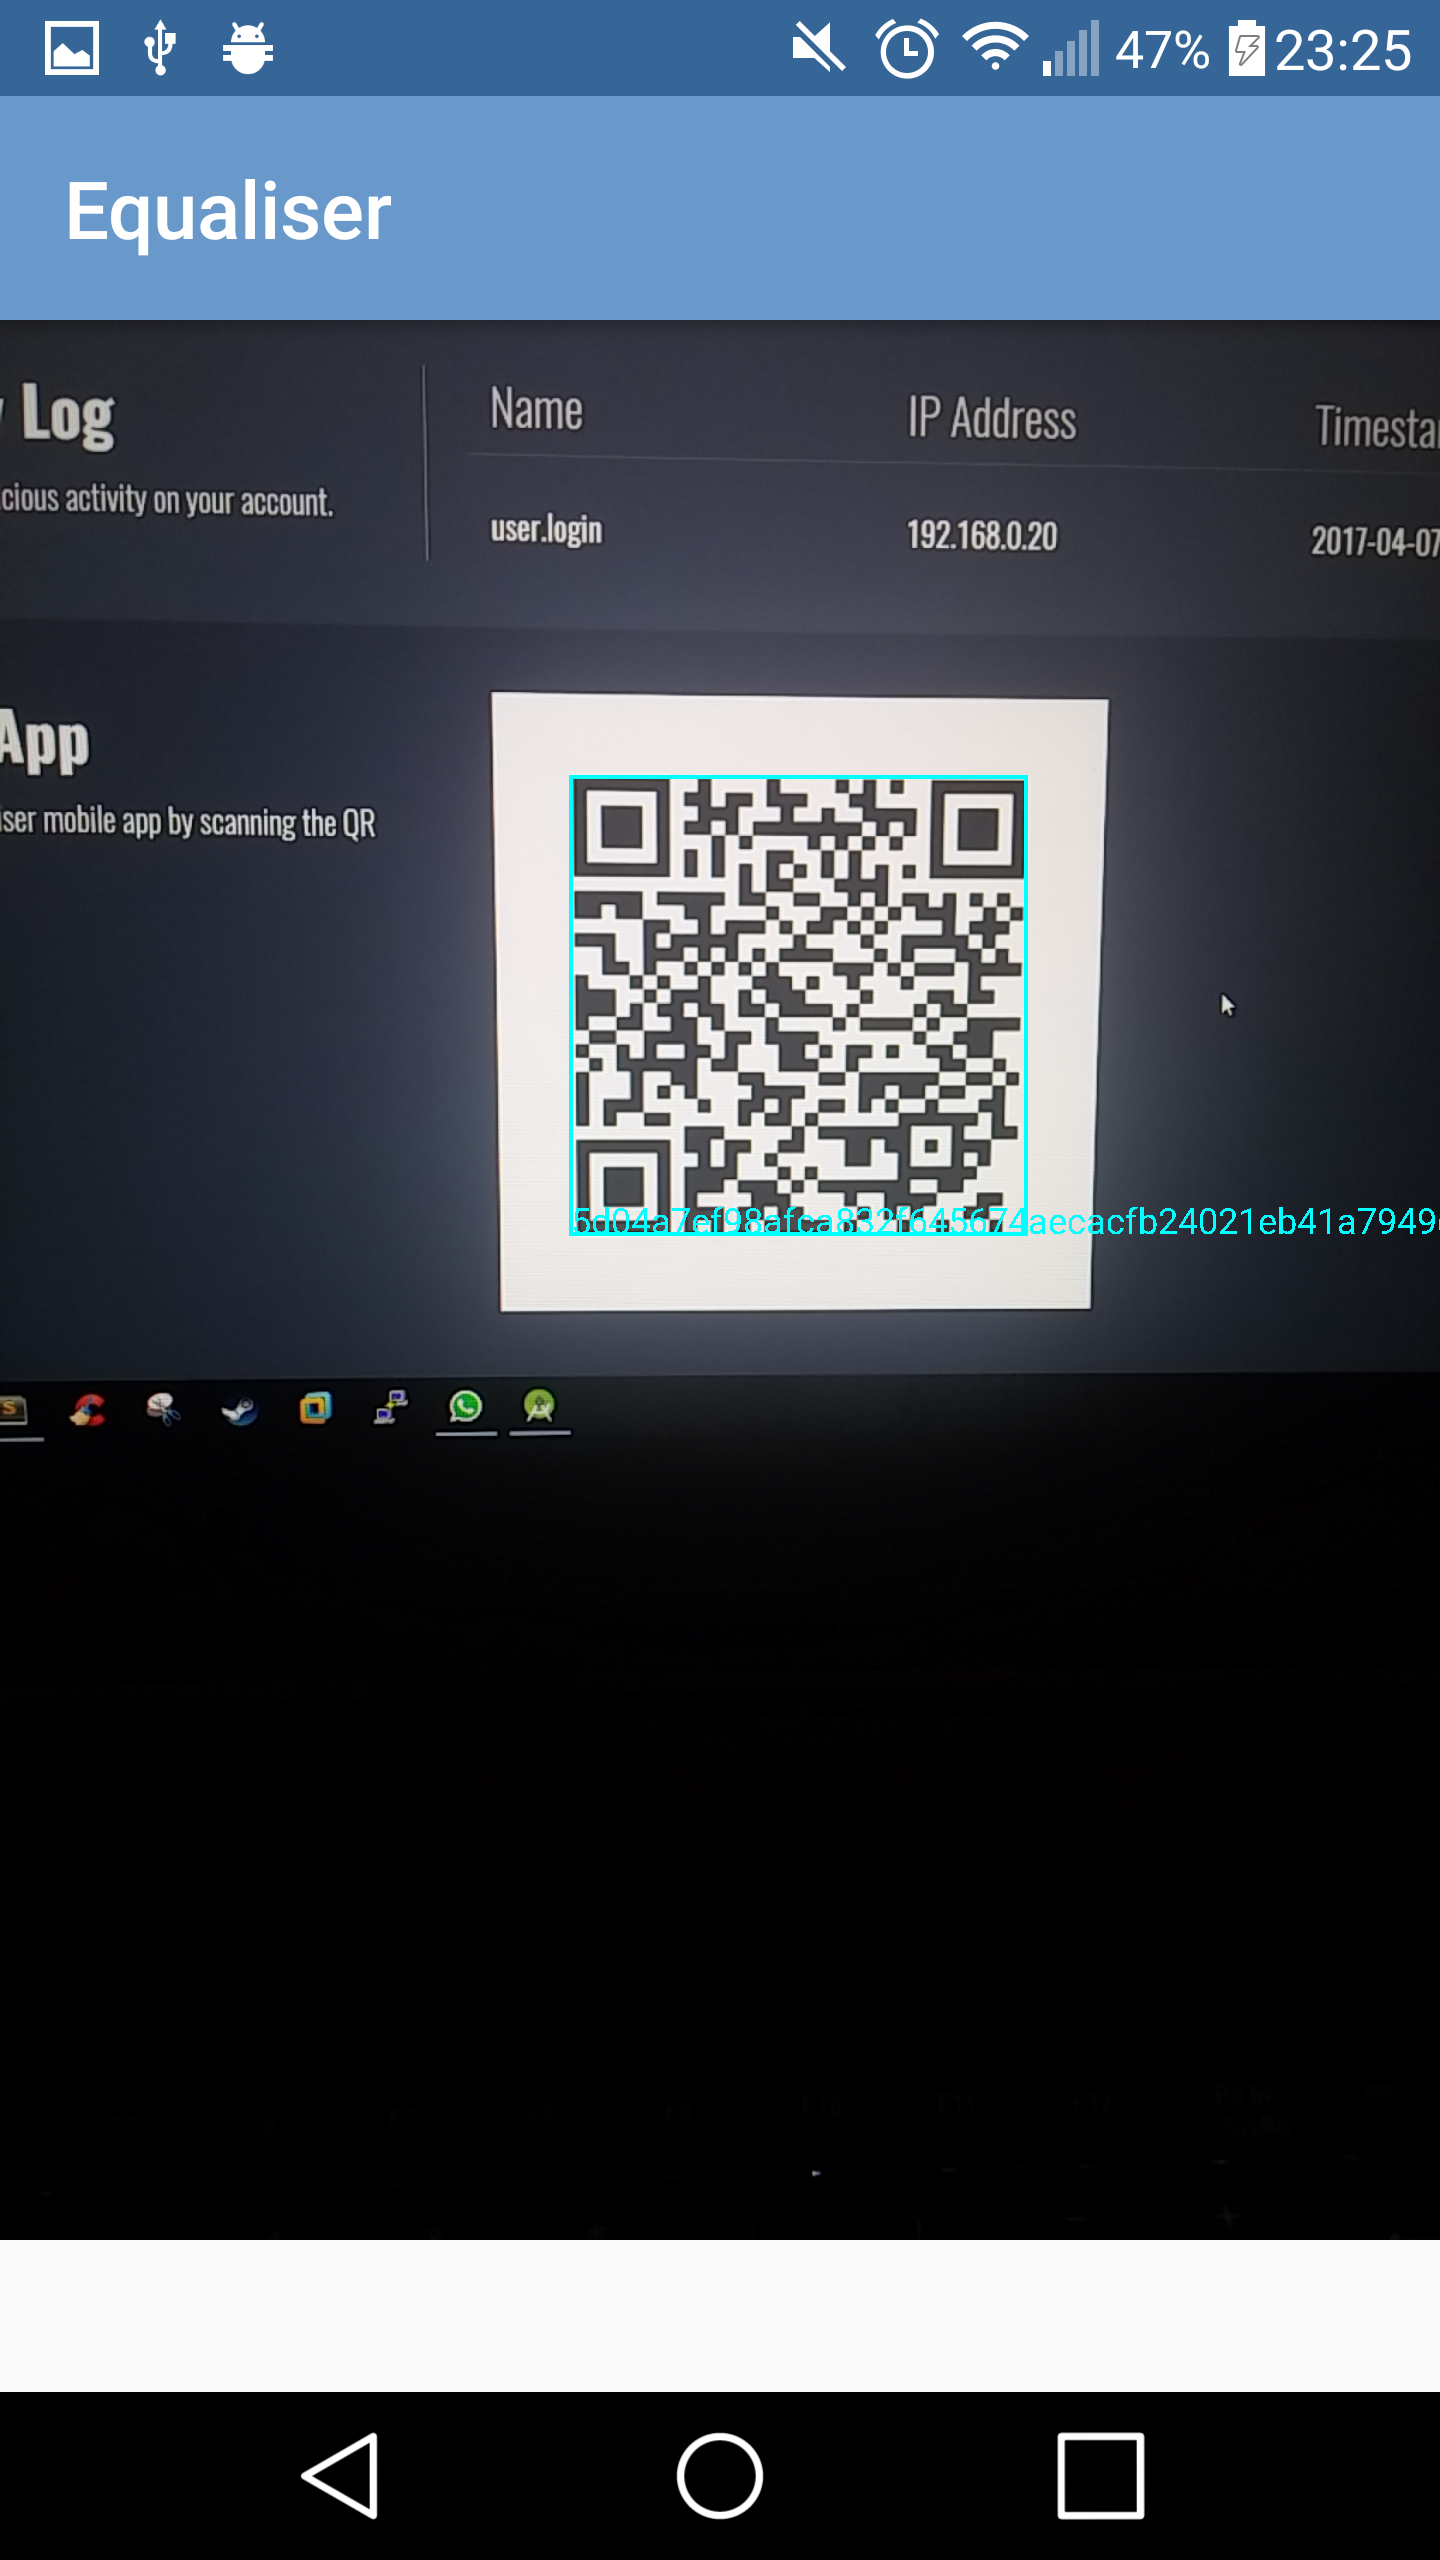
\includegraphics[width=\textwidth]{img/app_qr_scan.png}
    \caption{The mobile app while scanning an ephemeral token}
    \label{fig:app_qr_scan}
  \end{minipage}
  \hspace{0.05\textwidth}
\end{figure}

Once the app identifies the QR code and extracts the hex string, it sends a \code{POST} request to \code{\path{/auth/ephemeral}} containing only that string. On success, the API will respond with user and session information, allowing the app to display basic user details, as shown in Figure \ref{fig:app_left_menu}. To prevent getting stuck on the log in screen, the backstack is also cleared, so if back is pressed, the app quits.

\begin{figure}[!htbp]
    \centering
    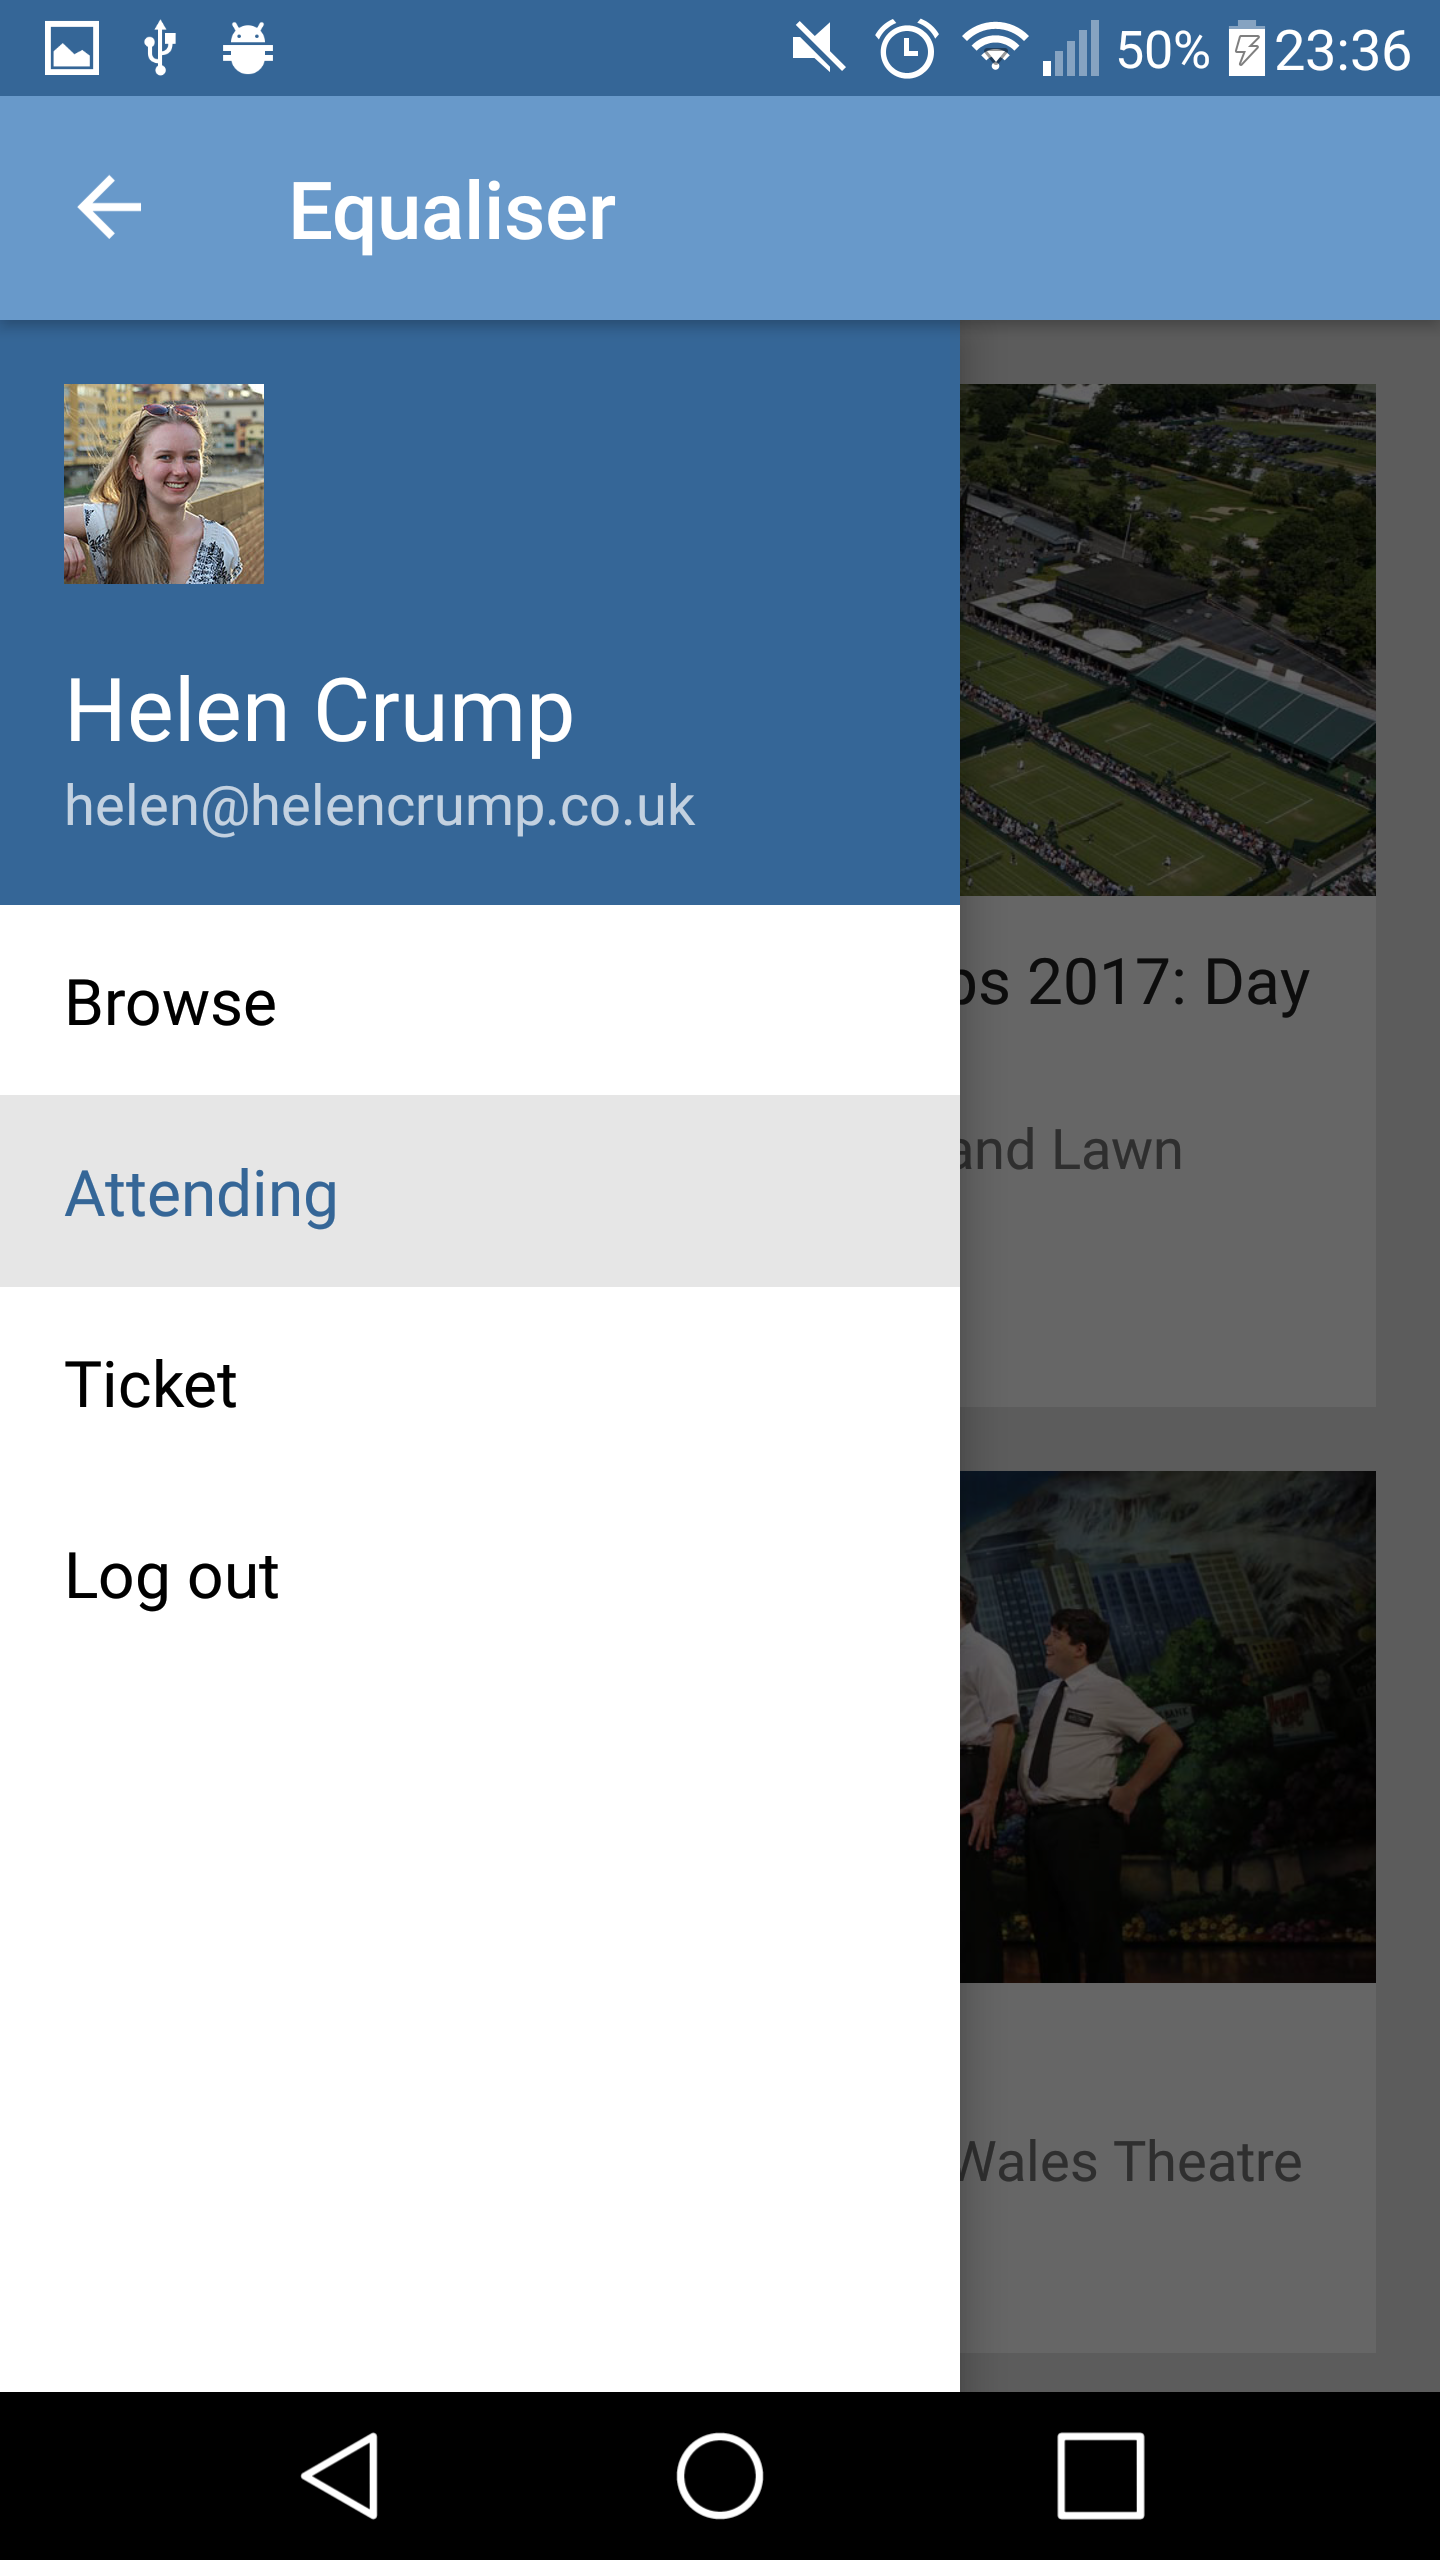
\includegraphics[width=.5\linewidth]{img/app_left_menu.png}
    \caption{The mobile app in its logged-in state, showing the left pull out menu}
    \label{fig:app_left_menu}
\end{figure}

To prevent having to go through this process every launch (which would be unworkable at venues), the app leverages Android's \code{SharedPreferences} persistence API to store the session token and user details. When it starts up, it checks for the presence of this token. If it exists, it knows the user is logged in and can proceed to the event showcase. Otherwise, it prompts to scan a new QR code. On log-out, the persistent storage and screen backstack are cleared to prevent a user simply pressing the back button to log back in.

\subsection{Ticket Display}

Displaying a ticket on a phone required rendering arbitrary data in a format that could be visually transmitted without losing accuracy. The well-known solution to this is barcodes. The majority of paper tickets use a 1D barcode which conveys a 12-16 digit number. Equaliser could have been easily satisfied by this, however the lack of parity and normalisation features (to account for size, orientation, angle of viewing etc.) meant that scanning across a range of screen sizes could be problematic. I knew QR codes had these features, and was about to implement them when I discovered Aztec barcodes. These can encode up to 1914 bytes of data while supporting Reed-Solomon error correction and viewing from any angle \cite{A14}. I only needed to encode 32 bytes of data, so was able to increase the amount of space used for parity. In fact, Aztec is specifically designed to produce readable codes on mobile phones. I used Google's ``Zebra Crossing'' library \footnote{\url{https://github.com/zxing/zxing}} to render these barcodes on the phone. An example of a rendered ticket can be seen in Figure \ref{fig:ticket}.

\begin{figure}[!htbp]
    \centering
    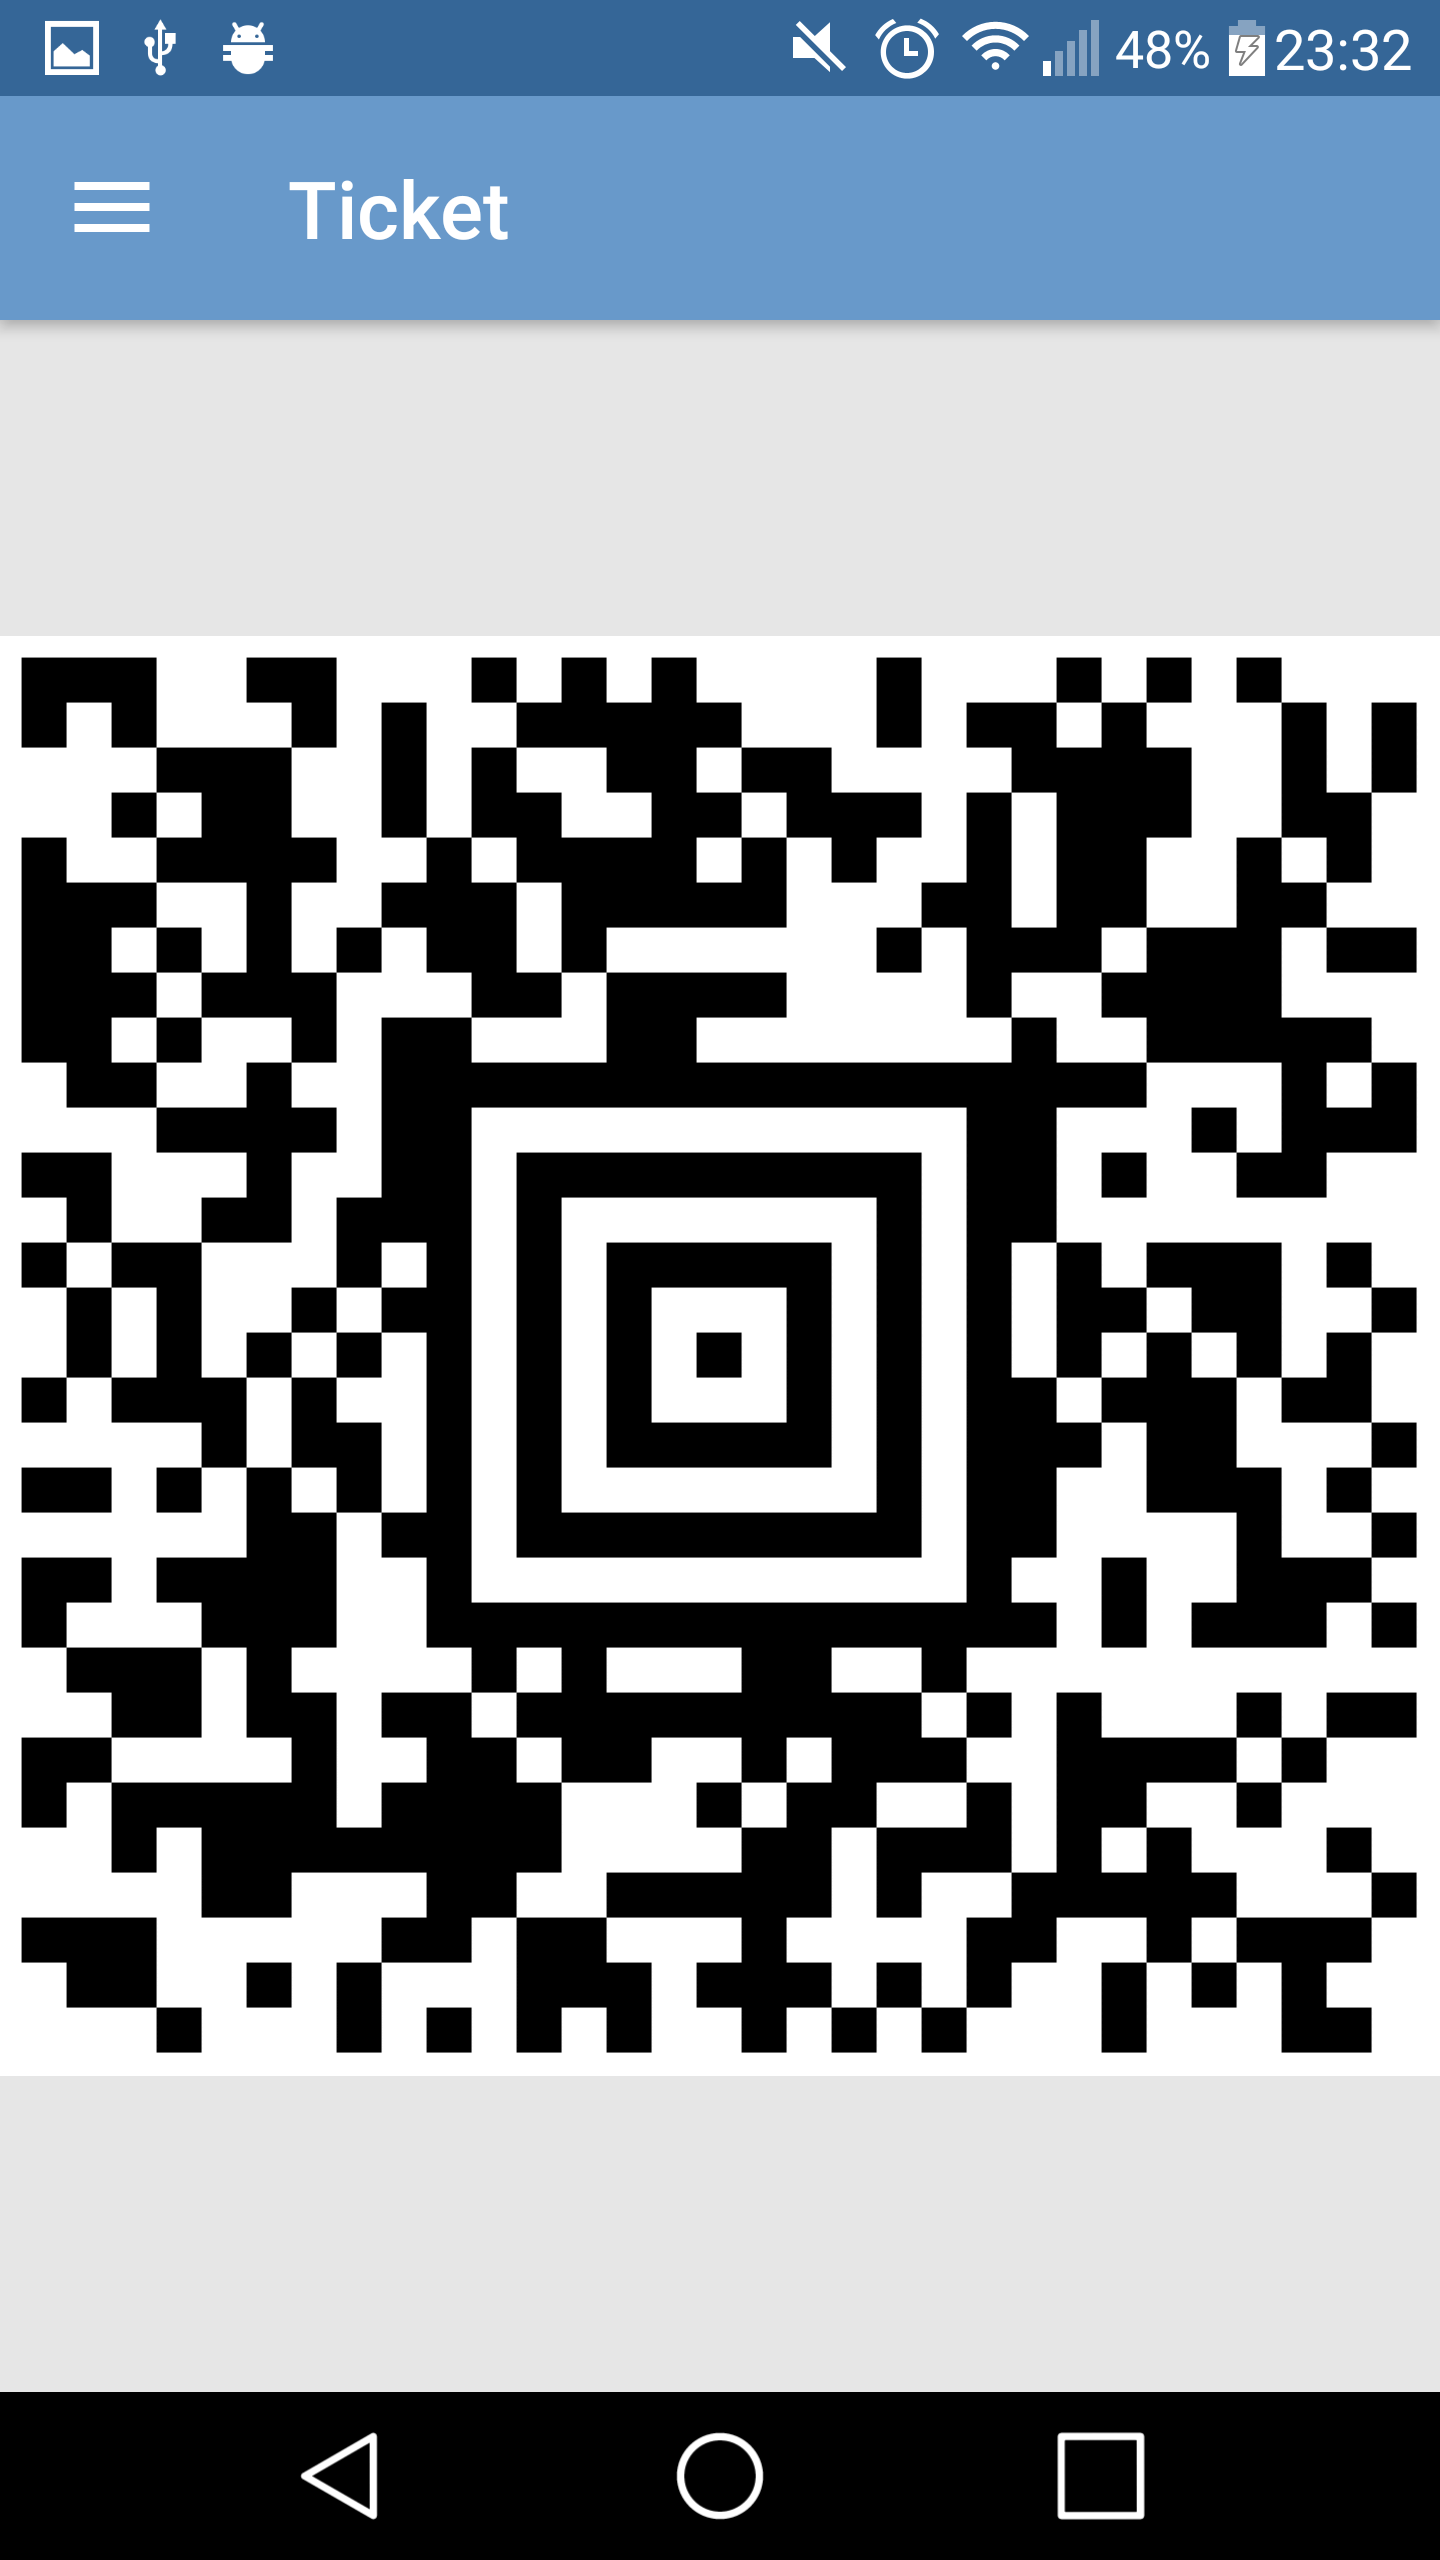
\includegraphics[width=.5\linewidth]{img/ticket.png}
    \caption{Ticket displayed in the mobile app}
    \label{fig:ticket}
\end{figure}

\section{Ordering Deep Dive}

% TODO include screenshots from mobile app and JSON responses

This section goes into the technical details of how different parts of Equaliser co-operate to fulfil demand for tickets. Firstly, a user clicks a wait or buy button in the web or mobile app. This takes them to the order form, shown in the website for an Elbow concert in Figure \ref{img:order}. As per the requirements, this allows the group leader to add other users. I implemented a simple auto-complete feature here to reduce errors and assist with entry, demonstrated in Figure \ref{img:order_autocomplete}. Pressing the enter key will confirm the selection, shown in Figure \ref{img:order_attendees}. Note that it is possible for the group leader to remove themselves via the ``Delete'' button next to their name, provided at least one other user is added first.

\begin{figure}[!htbp]
    \centering
    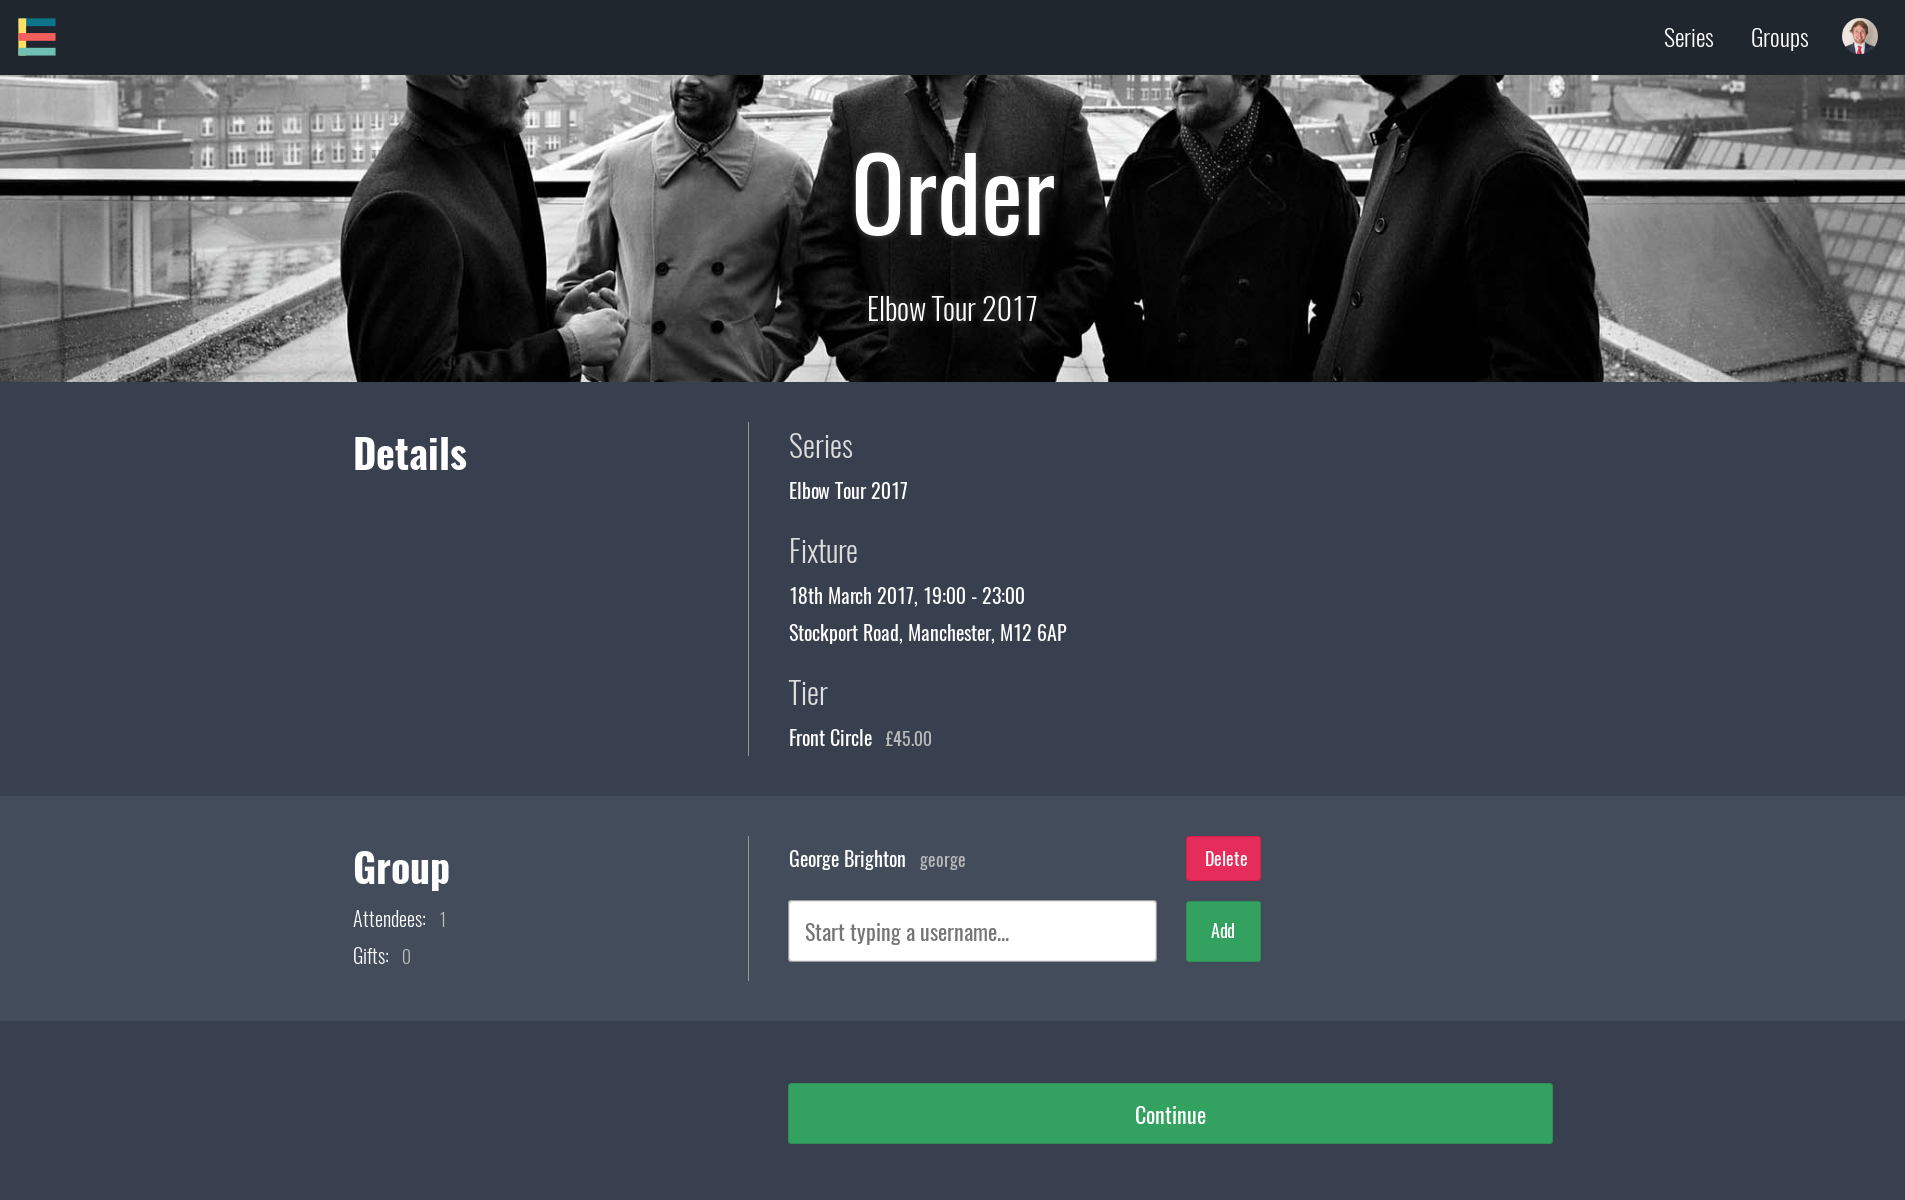
\includegraphics[width=1\linewidth]{img/order.png}
    \caption{The order page for a series}
    \label{img:order}
\end{figure}

\begin{figure}[!htbp]
    \centering
    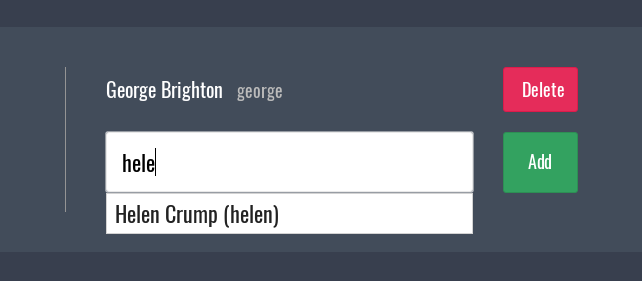
\includegraphics[width=1\linewidth]{img/order_autocomplete.png}
    \caption{User suggestions are offered after 4 characters are entered}
    \label{img:order_autocomplete}
\end{figure}

\begin{figure}[!htbp]
    \centering
    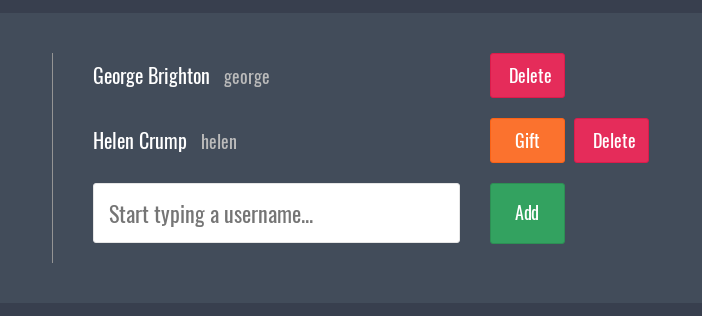
\includegraphics[width=1\linewidth]{img/order_attendees.png}
    \caption{Two users added to an order}
    \label{img:order_attendees}
\end{figure}

To designate an individual as a giftee, the ``Gift'' button can be clicked, which then greys out, as shown in Figure \ref{img:order_attendees_gifted}, to indicate the ticket will be charged to this account.

\begin{figure}[!htbp]
    \centering
    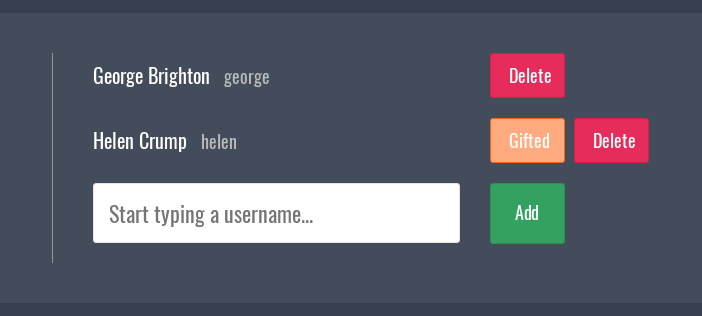
\includegraphics[width=1\linewidth]{img/order_attendees_gifted.png}
    \caption{A user selected as a giftee}
    \label{img:order_attendees_gifted}
\end{figure}

The user then clicks ``Continue'' to place their order. A client indicates intent to create a new order by sending a HTTP \code{POST} request to the \code{\path{/group/create}} endpoint. The naming inconsistency here is a result of ``orders'' not being a solid concept; a demand for tickets is implied by the existence of a group.

The web request is received in \code{RestVerticle}, which triggers a method assigned to that resource. This method first ensures the input makes sense, before marshalling it into objects (for example, raw usernames are turned into \code{User} objects which all accompanying attributes). More complex validations are then performed, for example to ensure no users in the group are already waiting for the event. This is also enforced at the schema level via a composite unique index constraint. Finally, it creates a \code{Group} object, and inserts this into the database, which behind the scenes involves inserting rows into a number of tables, all within a single transaction.

Instead of stopping here, for the benefit of clients, the handler immediately tries to reserve tickets for the group by sending a message over the event bus to \code{Primary\-Pool\-Verticle}. Verticles can register methods which listen at arbitrary addresses, which are simply \code{String}s. One such method exposed by this verticle is \code{primary\_pool.\-reserve}, which takes a tier identifier and number of tickets, and atomically checks whether that many tickets are available, and decrements the count by that number. It returns a boolean indicating whether the tickets were available.

This verticle is deliberately simple because it must be fast. The rest of the order process can scale out to infinity, however the specific part that deals with reserving tickets must be shared mutable state. Making the verticle simple allows it to be as fast as possible. If the verticle fails, it is always possible to reconstruct its hash table from the database. In practice, instead of a hash table, a system like Redis would be used to provide a more resilient store.

If the \code{Primary\-Pool\-Verticle} returns failure to reserve the tickets, the ordering system knows the tier must be sold out, and so allows the group leader to choose additional tiers they are interested in, which are stored in the \code{GroupTiers} table. Otherwise, the worker dealing with the order now knows it has permission to offer tickets to the group. Let's follow this main success scenario. An \code{Offer} object is created and inserted into the database, then included in the response:

\begin{minted}{json}
{
   "success": true,
   "result": {
      "group": {
         "id": 8,
         "leader": "{snipped}",
         "fixture": "{snipped}",
         "created": 1491821339.736,
         "status": "WAITING",
         "size": 2,
         "paymentGroups": [
            {
               "id": 9,
               "payee": "{snipped}",
               "attendees": [
                   "{snipped}"
               ],
               "status": "INHERIT"
            }
         ]
      },
      "offer": {
         "id": 7,
         "tier": {
            "id": 14,
            "name": "Front Circle",
            "price": 45,
            "availability": 1000,
            "fixtureId": 4
         },
         "timestamp": 1491821339.764,
         "expires": 1491821939.764
      }
   }
}
\end{minted}

It is important to note that the ``waiting list'' is completely implicit. Having a queue of orders would incur too many writes to be efficient, so instead all allocations are done in the background while users are not waiting for a response. The \code{OfferIssueVerticle} first checks the number of tickets in secondary pool. If it is greater than 0, the daemon tries to give offers to those in the waiting list. If it exhausts all available tickets and the waiting list is still not empty, it will try to process refunds equivalent to up to 50\% of the number of tickets required by the waiting list, in order to fulfil the demand. It does not process 100\% of the required number, as offers will be constantly expiring (and collected by the \code{OfferReclaimVerticle} and put in the secondary pool), and demand may stop at any time. If Equaliser processes refunds too quickly, supply will rise above demand, and revenue will suffer.

Payment group leaders will now receive a text message notifying them of their offer, similar to the one shown in Figure \ref{img:offer_notification}. The website also displays a countdown to the \code{expires} time, as in Figure \ref{img:offer}.

\begin{figure}[!htbp]
    \centering
    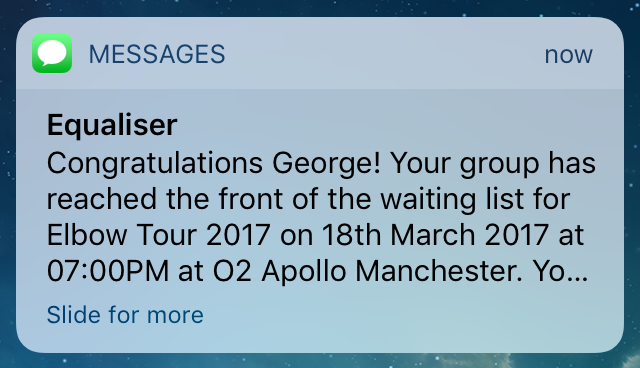
\includegraphics[width=.6\linewidth]{img/offer_notification.png}
    \caption{SMS notification of an offer}
    \label{img:offer_notification}
\end{figure}

\begin{figure}[!htbp]
    \centering
    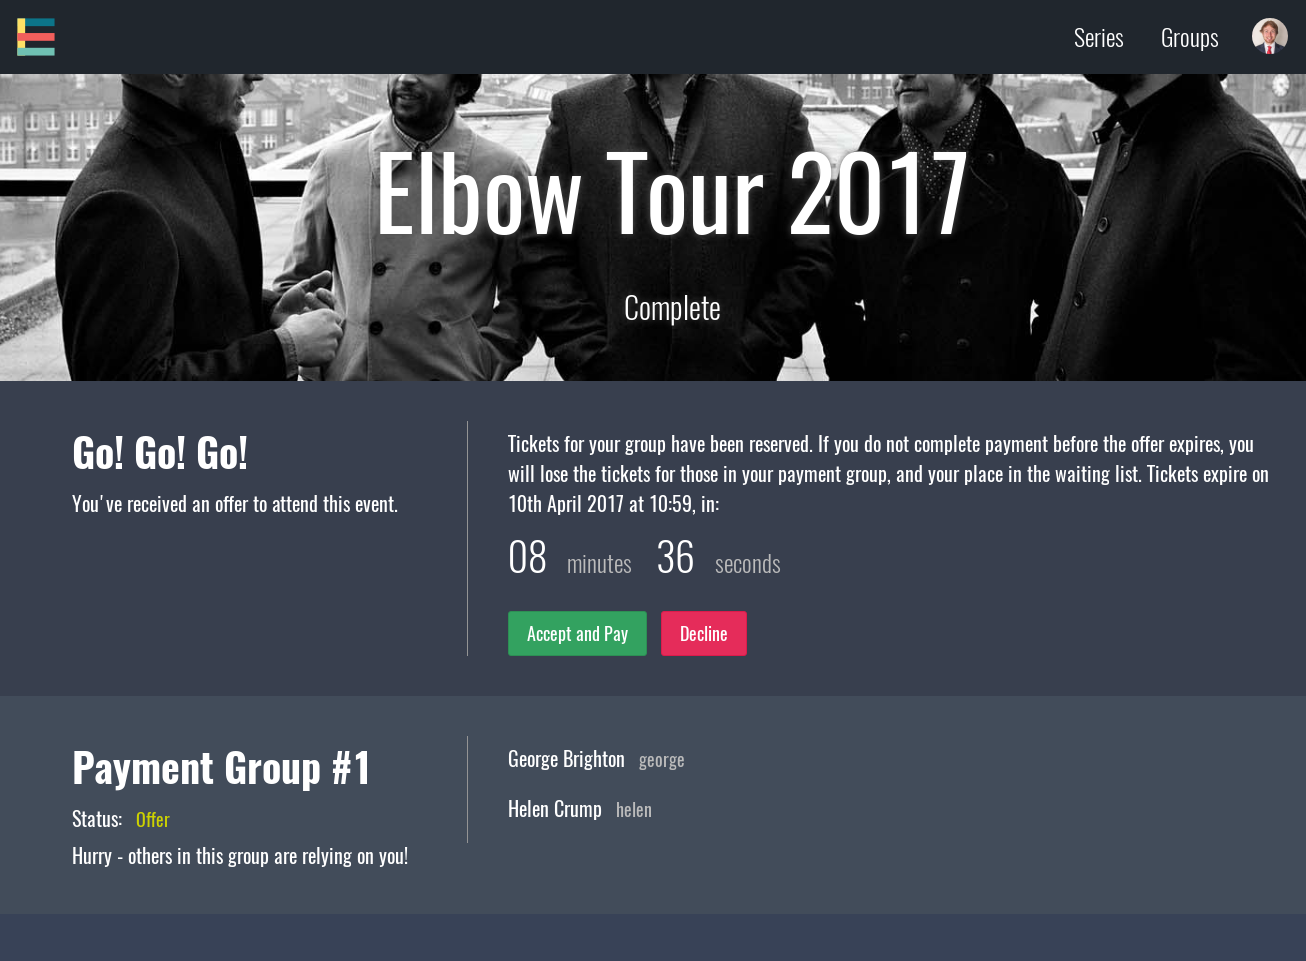
\includegraphics[width=1\linewidth]{img/offer.png}
    \caption{A payment group leader showing an offer for tickets}
    \label{img:offer}
\end{figure}

A client pays by sending payment details in a \code{POST} request to \code{\path{/group/:id/pay}}, where \code{:id} is the unique group identifier. The system automatically identifies the payment group the requesting user is responsible for, and registers the payment against that. Assuming this is completed in time, a transaction and tickets will be created for everyone within the payment group, and the user will receive a confirmation similar to the one shown in Figure \ref{img:going}.

\begin{figure}[!htbp]
    \centering
    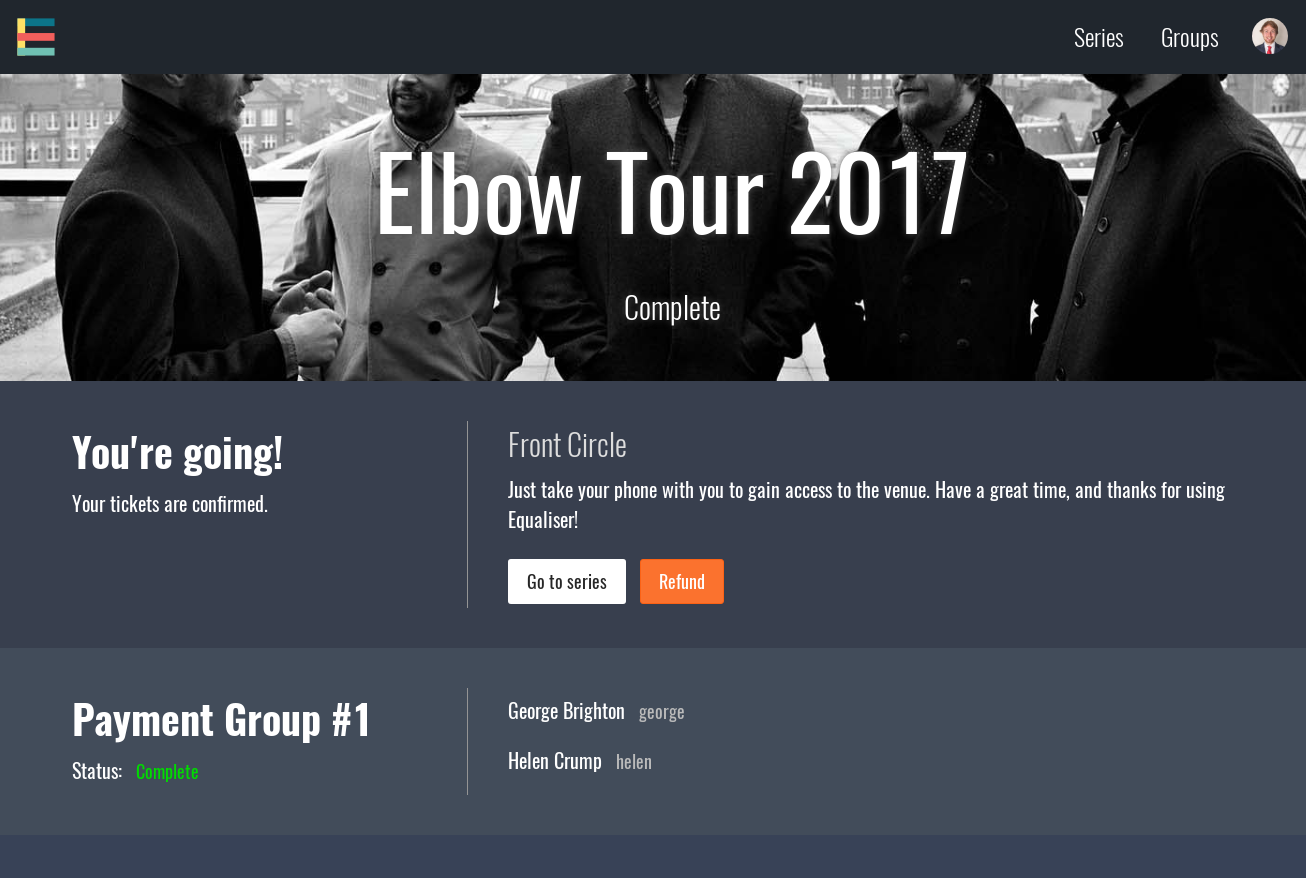
\includegraphics[width=1\linewidth]{img/going.png}
    \caption{Payment confirmation for a payment group leader}
    \label{img:going}
\end{figure}

Within 30 seconds, \code{TicketNotificationVerticle} will pick up the completed payment group, and send notifications resembling Figure \ref{img:ticket_confirmation} to all attendees within it.

\begin{figure}[!htbp]
    \centering
    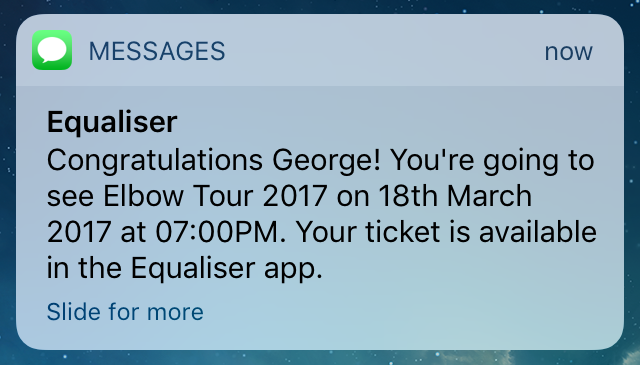
\includegraphics[width=.6\linewidth]{img/ticket_confirmation.png}
    \caption{SMS notification of a completed order}
    \label{img:ticket_confirmation}
\end{figure}

Now, attendees simply wait for the fixture. The status of other payment groups can can be seen on the order page so friends in a group know who they are attending with. All go through the same process of the payment group leader being alerted. If any payment group leader does not complete their transaction before the offer expires, attendees in their payment group will lose tickets, however they are able to place a new order. The SMS notifications are designed to allow individuals to hold their payment group leader responsible when they receive an offer. A high-level overview of the process can be seen in figures \ref{img:order_state_diagram} and  \ref{img:order_interaction}.

\begin{figure}[!htbp]
    \centering
    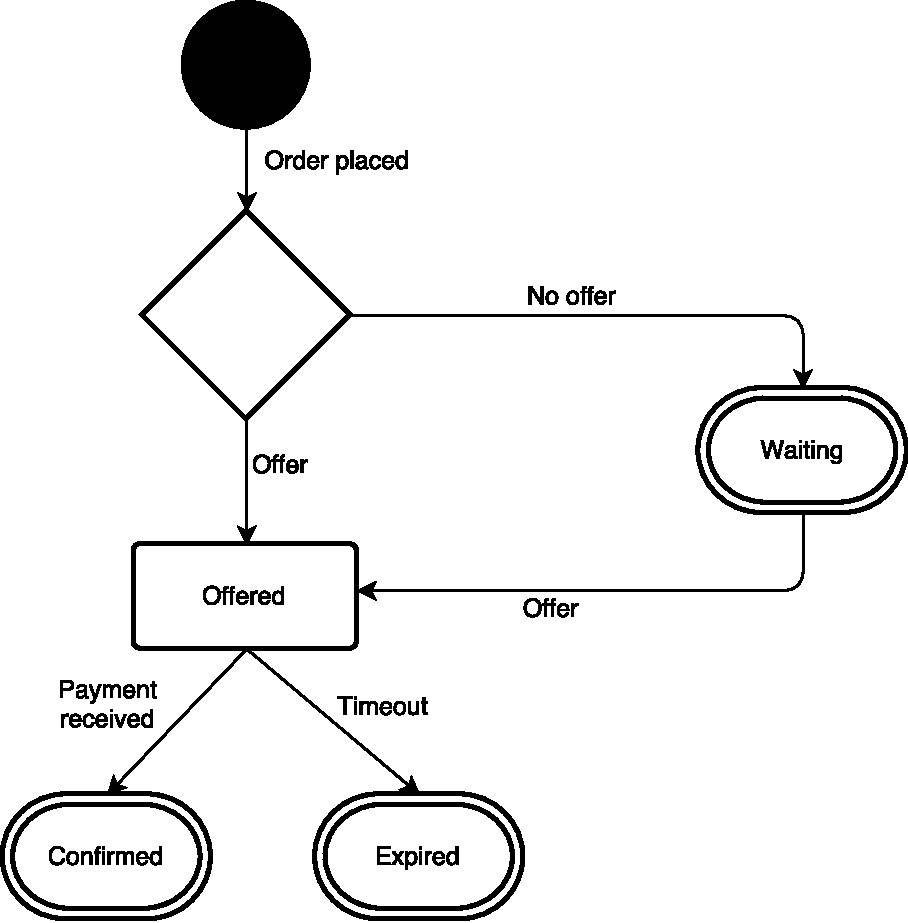
\includegraphics[width=0.8\linewidth]{img/order_state_diagram.pdf}
    \caption{High-level state machine diagram of ordering process}
    \label{img:order_state_diagram}
\end{figure}

\begin{figure}[!htbp]
    \centering
    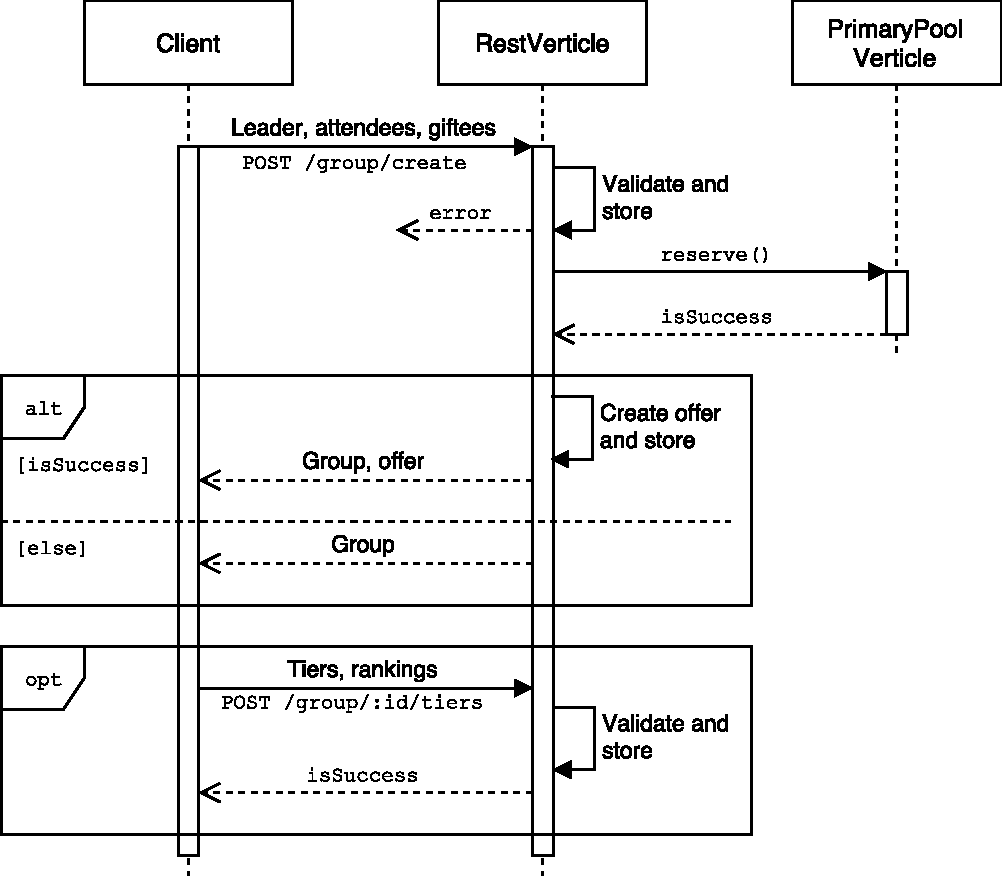
\includegraphics[width=0.8\linewidth]{img/order_interaction.pdf}
    \caption{Interaction diagram detailing a typical order}
    \label{img:order_interaction}
\end{figure}

\chapter{Testing} \label{testing}

Given the time spent in the design phase, I knew the requirements for each class that made up the API, and so could broadly follow a test-driven development workflow. This chapter details my testing strategy, and difficulties I encountered.

\section{Asynchronous}

I ran into a seemingly serious issue in the very first test case I wrote. Unit tests are run synchronously, whereas the API is entirely asynchronous. Fortunately, Vert.x has a \code{vertx-unit} artefact that is designed for testing such code. It seems to be a fusion of Vert.x and JUnit.

Each unit test receives a \code{TestContext} object, which has an \code{async()} method, returning an \code{Async} object. Calling this method marks the test case as executing. The test framework only knows the test case has terminated if and when the \code{Async}'s \code{complete()} method is called. In practice, this made testing a little more awkward, as all code paths within a test case had to finish with a call to \code{async.complete()}. Forgetting this would result in a non-terminating test.

As a simple illustration, the following test case ensures the \code{GET /countries} endpoint returns a success response. Further validation would be needed to ensure the actual data returned was valid.

\begin{minted}{java}
@Test
public void testGetCountriesSuccess(TestContext context) {
    final Async async = context.async();
    vertx.createHttpClient().getNow(
            PORT, HOST, "/countries", response -> {
        response.handler(body -> {
            JsonObject json = new JsonObject(body.toString());
            context.assertTrue(json.getBoolean("success"));
            async.complete();
        });
    });
}
\end{minted}

\section{Continuous Integration}

Unfortunately, I did not have the resources to configure a GitLab Runner, so as a workaround, I configured my project repository with an additional remote pointing to GitHub, and adopted the workflow of pushing to GitHub, waiting for Travis CI to run the test suite, then pushing to GitLab if all tests passed. Vert.x's ability to generate a fat \code{.jar} via the \code{shadowJar} Gradle plugin meant running tests was simply a case of building the project and executing a single command.

\section{Linting}

I ran IntelliJ's code inspections many times throughout the project, which helped flag up overly-open access modifiers, unused variables and missing parameter JavaDoc. While I doubt these tools actively prevented any bugs, they certainly maintained a high standard of code hygiene.

\chapter{Evaluation} \label{evaluation}

This chapter quantitatively evaluates Equaliser, attempting to ascertain how well it fits the requirements and needs of the stakeholders that would use it. I am happy that all functional and non-functional requirements were met.

\section{Comparison}

This section compares Equaliser with other ticket distribution systems, highlighting its key advantages and weaknesses from the perspectives of various stakeholders.

\subsection{Attendees}

Unlike the biggest players in the industry, Equaliser does not charge any fees on top of ticket prices. All customers see one price per tier. The same is true for refunds, which are automatic and free. A possible bugbear to consumers is the presence of the ``reallocate'' refund policy, however this is no worse than any other system.

Attendees can rest assured that the queuing system is fair, with no touting possible. Everyone in a group knows exactly where they stand, and whether they have received an offer for tickets.

On the day of the event, customers do not need to bring any additional identification with them, reducing appeal to thieves. Those too young to own a payment card are no longer disadvantaged, and ticket gifting is much less painful as an additional benefit. At the venue itself, unlike any other system, groups no longer need to wait for everyone to arrive before passing through the ticket barrier.

\subsection{Venue}

While in theory, Equaliser does not place any more responsibility on venues, due to paperless ticketing requiring photo ID, in practice, they do not do this, and Equaliser falls to pieces if faces are not matched to those on record when entering the venue. Although the tokens used to generate barcodes are kept secret, they are not designed to protect against copying. If photo ID is not verified, anyone can use a given barcode to enter an event. Allowing users to simply scan their token offers similar security to the ticketless process today.

Equaliser allows venue management to hire fewer staff, both due to eradicating the need for a box office, and by permitting a single barrier attendant to verify multiple lanes of people simultaneously. All other systems on the market currently require manual verification of tickets and identity in person, and cannot easily be altered.

\subsection{Organiser}

Organisers no longer have to worry about the Consumer Rights Act 2015 \cite{H15}, as Equaliser handles all ticket refunds and redistribution. Even if an organiser decides to build their own front-end store for the API, there is no reason to hide the location or face value of resold tickets, as it is guaranteed to always be the same for any given tier.

Equaliser neutralises bots, and removes the need to limit the size of groups, potentially allowing events to sell out more quickly. This comes with no disadvantage, as the organiser can rest assured that a person can only have one ticket, and they were named before payment, so there is no possibility of touting. Tickets prices could even be raised slightly, as inclusive fees give the illusion of being cheaper for customers through lack of additional charges.

\section{Assurance}

There are no known serious vulnerabilities in Equaliser's practical design. The following are hypothetical situations imagined during the design phase that were deemed too unlikely or difficult to achieve to be concerned about. By accepting these risks, Equaliser was able to achieve higher security in other areas.

If a group of malicious actors bought tickets, they could co-ordinate returning them at the same time to rapidly pop people from the waiting list. For example, if someone really wanted to attend an event, they may be willing to pay someone £10,000 to return 30 tickets. Equaliser defends against this by not revealing positions of those in the queue. I do not believe anyone, even the most desperate of fans, would pay large sums of money on the off chance of getting to the front of a queue. Fortunately, the most die-hard fans tend to want to attend the largest events, which by definition will have more demand and a longer queue, making this attack infeasible.

Although not considered for Equaliser's threat model, there is nothing to stop an individual creating a service that offers to buy people's tickets on their behalf immediately after purchase. This is a fork of the automated purchasing problem. The person could prepare the necessary web requests, and fire them off at the first opportunity in an effort to beat all other demand. This is not strictly touting, as there is no transfer of ownership happening, but it would allow a service to charge arbitrary fees to desperate fans, and give them an unfair advantage. In practice, the best defence against this attack is likely to be setting up honeypots that ban users trying to use them, or analysing traffic to the API, looking for users who seem to always order tickets in the seconds just after release, before they could reasonably complete the order form. It could also be interesting to look for orders originating from ranges of IP addresses not registered to consumer ISPs, that reserve tickets for a seemingly unrelated group of people. It is also possible to imagine a scenario where a group of dedicated fans have purchased software to buy their tickets, however again it would leave a trace, and arguably these are fans who simply really want to attend the event. I considered side-stepping the problem by setting up a ``priority'' queue in Equaliser, allowing users to pay more for guaranteed tickets and effectively stealing the business, however this would earn the system bad publicity, and is unfair to genuine fans.

Crucially, Equaliser does not have to be completely watertight in order to discourage touts; it only has to cause them enough inconvenience that it is no longer a viable business. A customer will only buy a ticket from a tout if there is a sufficient probability of it being accepted. If this probability is too low, touts will simply disappear. Equaliser aims to keep that probability as low as possible, and provided venues are diligent in verifying the identity of those who show up, it is close to 0. The only way to fool the system is to look convincingly like another individual who has a ticket, and also know their token.

\section{Security}

Aside from ticket security, Equaliser offers several other mechanisms to protect users' interactions with the service. As detailed in section \ref{tech_design_api_authentication}, all login attempts must go through the two-factor authentication process. While secure, this could still be improved. Sending a text messages costs \$0.04 \cite{T17}, and there are non-trivial costs associated with renting the numbers themselves, and messages are limited to 10 messages per second. Even so called ``short codes'', which are intended for high-volume messaging, can only send 100 messages per second, and cost \$20,000 per year \cite{T17}. This could become a significant cost, as multiple of these are likely to be needed due to logins spiking during ticket releases, and in the hours before events. A cheaper and more modern solution could be to use the native Android push notification service, called Firebase Cloud Messaging, which is free for any number of notifications. Given more time to register for Firebase, I would use that as the primary second-factor mechanism. SMS messages would be required as a fallback, but operating costs would be significantly reduced.

All requests to the Equaliser API and website can be wrapped in TLS. I did not implement this, as in practice, this would be terminated at the load balancers, so the service would only see raw HTTP. The website itself has protection against cross-site scripting and request forgery. The Django library and Jinja template language make this trivial to implement with a few lines of code. The API is not susceptible to such attacks as an \textit{Authorization} header must be included for all requests that mutate state.

To help users help themselves, there are no restrictions on valid password characters. Bcrypt is used in the backend with $2^{10}$ rounds, which results in hashing taking roughly 600ms on my hardware. If Equaliser were moved to a higher performance server, this number could be increased to offer more security, until the time it took to verify and generate hashes was too great from a user-experience perspective.

\section{Efficiency and Maintainability}

Unfortunately, due to investment in the design phase, I did not have time to performance test the system, using JMeter or an equivalent tool. However, due to the asynchronous way Equaliser is implemented, I can say that it makes very efficient use of the hardware it is on. Indeed, the entire application, including background tasks, was perfectly responsive running on a single logical core on my laptop, with the database on another.

By implementing two API clients, I have shown that the API works generally, and its simplicity is a testament to the amount of time I spent in design. My technical decisions were so suitable because I had all the information I needed to make them, so I would not necessarily spend my time any differently were I to complete another similarly uncharted project again.

\section{Development Methodology}

Agile methodologies are vastly preferred nowadays, however I found they were not suited to this project, at least at a macro level. Equaliser depends on each part of the ordering process being secure both individually and together, whereas an agile development cycle necessitates rapid self-contained iteration. If I had fully implemented a feature each time I had an idea, the amount of refactoring would be equivalent to rewriting the project several times. Managing expectations by producing a minimum viable product would not have worked in the case of Equaliser.

Instead, I needed to take a high-level approach more similar to waterfall during the design phase. Within each component, for example the ticket barrier client, there were traces of a more modern methodology, such as iterating to reduce costs and improve customer experience, however the security of the overall product is too coupled to develop, say, the ordering process and venue entry systems in isolation. Agile works best when the project design is relatively straightforward or at least well-known. Equaliser is neither, with the vast majority of time spent in the design phase, and development only taking several weeks.

Before firing up an IDE, I needed a solid specification and a plan for avoiding gaping holes. One cannot implement hacks in a practical design in the same way it is possible to in code. Such patching leads to very real irritation, like limits on group sizes, and reCAPTCHAs. Having this detailed plan meant the programming part of this project was almost trivial.

\section{Personal Reflection}

Aside from the opportunity to learn Vert.x and Android development, I found the project incredibly interesting and useful on many levels. On one hand, it is just a student's final project, but on the other, I can genuinely see how such a system could be deployed and used by tens of thousands of people, which is incredibly satisfying.

\subsection{Surprises}

The key difficulty and most interesting part of the project was the practical design. I spend many hours exploring ideas, refining them, then realising my assumptions were incorrect in increasingly subtle ways, meaning solutions would not work - which is surely a sign of progress. Gifts and groups, particularly on the waiting list, were a significant source of complexity in the database, however requirements are just that, and I enjoyed the challenge of finding elegant solutions by avoiding problems altogether. I have never had the opportunity to solve problems both at the human level for the system design, and at the code level for turning that design into a working piece of software before. This kept the project interesting, as it was not simply a question of typing. 

The second surprise, however pompous it may seem, is just how idiosyncratic libraries can be. From Vert.x's decision to pass prepared statement parameters in a \code{JsonObject}, to Android's Volley library's \code{JSONObjectRequest} seemingly not supporting \code{POST} request parameters, not being used to these APIs highlighted every jagged edge in them. There were also a number of hideous bugs and omissions, for example Vert.x crashing if it receives an empty \code{POST} field name, and only returning the first inserted primary key when multiple rows are inserted. I have a long list of pull requests upon the conclusion of the project.

\subsection{Roadmap}

As with any project, there are an infinite number of ways in which Equaliser could expand. I regret not having time to try out more professional tools like DropWizard and Elasticsearch. In particular, I would have liked to create a real-time dashboard showing events, free seats, the rate of sales, size of the waiting list and churn, waiting list acceptance rate and so on. It could have been implemented in many fascinating ways, however it would ultimately have just been a programming challenge, so I am glad I focused on the more difficult human problem of touts.

\chapter{Applications} \label{applications}

Equaliser was designed to be able to handle ticket distribution for entertainment events, however there is no reason why this cannot be expanded. This section explores the use of Equaliser as a platform, and potential pitfalls.

\section{Design}

Equaliser ensures fair access to highly contended events. Everything it does relies on demand exceeding supply. Its primary drawback is the requirement for human verification, meaning it is not suitable for use in situations where ticket checking absolutely \textit{must} be automatic, at the cost of less security. There is no reason to have a waiting list or verify identities if supply is unlimited. Equaliser would therefore not be suitable for use on the London Underground, or to manage ski lift access for example. It would be very suitable for flights, where this checking is compulsory by law, however plane tickets neither suffer from contention nor touting issues, so it would be of limited use.

\section{Modularity}

Recall that Equaliser is in fact three components: an API, a mobile app and a website. Any extensions can freely pick and choose which of these systems to use with no modification required, drastically reducing the time and money required to introduce the platform. If a major artist wanted to sell tickets for their event using the Equaliser platform, but wanted to put their own shop on the front, that is easily possible by just using the API, with no security penalty.

\section{Scalability}

As Equaliser is modular not only at the component level, but also within the API itself, it is able to scale out by simply increasing the quantity of each verticle that is started. As already mentioned, the only fundamentally contended part of the system is ticket allocation, however this is mitigated by it being dedicated to that one task, and Redis can be swapped in should demand increase considerably. Implementing a CDN for resources would also be fairly straightforward due to the API explicitly returning all URLs, for example series images for the website.

\section{Possibilities}

Following on from my inspection, I looked into how Equaliser could be used to prevent the reselling of advanced Deutsche Bahn train tickets closer to the date of travel, undercutting the company. It appears that online ordering is locked down fairly capably, as names of all passengers must be specified at the time of booking, and cannot be changed afterwards. The key weakness is that tickets bought at machines do not require any form of identity, and can be purchased with cash \cite{D15}. These are easy to tout for the same reasons that any anonymous paper tickets can be resold.

Equaliser could potentially be used by Deutsche Bahn to handle the purchasing of tickets. In addition to preventing reselling, this would also remove the requirement for groups to travel together \cite{D17} and associated fees and credit card surcharge \cite{D171}. The company already has apps for iOS and Android, providing many useful features related to journey planning and delay notifications, which are too specific for Equaliser. However, Equaliser's decoupled architecture would mean that Deutsche Bahn could integrate their apps with both their own API, and Equaliser's, to provide both services simultaneously.

On the trains themselves, guards would need a scanner to verify the ticket barcodes. Unfortunately, this would not be reusable from the entertainment industry, however it would not be difficult to develop a new app for their use to interpret these codes - indeed, the Equaliser mobile app already does this for co-operative authentication. Effort would have to be put into locking down access to these endpoints however; arbitrary users cannot be allowed to pull users' profile photos and information.

Thinking more broadly, there is no reason why a similar system could not be applied to Virgin Trains and others in the UK. Fare dodging costs the industry £200M per year \cite{BM16}, with unscanned tickets often handed to others to use. It would be impractical to scan all passengers, but longer journeys naturally incur greater fees, and these are the ones that Equaliser would protect. Another mobile app could be built for customers that asks users to register railcards and other discount material, then automatically applied these to tickets bought.

\chapter{Conclusion}

Equaliser is a complete solution to the problem of ticket touting. My analysis uncovered desirable properties of systems resistant to touting, and I managed to achieve every single one of them. Equaliser reduces the amount of pressure put on customers while ordering tickets for highly sought after events, ensuring they can be safe in the knowledge that no one is unfairly jumping the queue. The system is capable of scaling to accommodate an indefinite number of users, while efficiently utilising whatever hardware it is running on. It is certainly the equaliser I hoped it would turn out to be.

\appendix
\begin{appendices}

%\chapter{API Reference}
%\label{appendix:api_reference}
% Methods, parameters and return values for the Equaliser API.

\chapter{Source Archive}
\label{appendix:source_archive}

Here's what's included and how to run it.
% TODO

\end{appendices}

\cleardoublepage  % http://tex.stackexchange.com/a/23503
\addcontentsline{toc}{chapter}{Bibliography}
\Urlmuskip=0mu plus 1mu
%\nocite{*} % can add back in to trivially increase page count
\printbibliography

\end{document}
